%===========================================================================
%generation of assignment and solution in one .tex file. make sure that write18 is activated(--enable-write18 for example as you call pdflatex.exe)
\gdef\conditionmacro{2}
\ifx\conditionmacro\undefined 
\immediate\write18{%
	pdfLaTeX --jobname="presentation_handout"
	\gdef\string\conditionmacro{1}\string\input\space\jobname
}%
\immediate\write18{%
	pdfLaTeX --jobname="presentation_with_notes"
	\gdef\string\conditionmacro{3}\string\input\space\jobname
}%
\gdef\conditionmacro{2}
%\expandafter\stop
\fi
%---------------------------------------------------------------------------

\ifnum\conditionmacro=1 \documentclass[handout,usenames,dvipsnames]{beamer}\fi
\ifnum\conditionmacro=2 \documentclass[usenames,dvipsnames]{beamer} \fi
\ifnum\conditionmacro=3 \documentclass[notes,handout,usenames,dvipsnames]{beamer}
\usepackage{pgfpages}
\setbeameroption{show notes on second screen=left} \fi
\usetheme{Boadilla}

%This file contains all packages and relevant definitions coming with them
%To use it add %This file contains all packages and relevant definitions coming with them
%To use it add %This file contains all packages and relevant definitions coming with them
%To use it add \input{../HEADERFILES_FOR_LATEX/PACKAGES} to the head of your file

%----------------------------------------------------------------------------------------------
%Typesetting
%----------------------------------------------------------------------------------------------
\usepackage[utf8]{inputenc} %To allow typesetting öäü

%----------------------------------------------------------------------------------------------
%Typesetting code
%----------------------------------------------------------------------------------------------
\usepackage{listings} %To allow nice typesetting of code

%Usage:
%Definition of all parameters defining the appearance of your code
%\lstset{ 
%	language=Matlab,% choose the language of the code
%	basicstyle=10pt,% the size of the fonts that are used for the code
%	numbers=left,% where to put the line-numbers
%	numberstyle=\footnotesize,% the size of the fonts that are used for the line-numbers
%	stepnumber=1,% the step between two line-numbers. If it's 1 each line will be numbered
%	numbersep=5pt,% how far the line-numbers are from the code
%	backgroundcolor=\color{SilverP},% choose the background color. You must add \usepackage{color}
%	showspaces=false,% show spaces adding particular underscores
%	showstringspaces=false,% underline spaces within strings
%	showtabs=false,% show tabs within strings adding particular underscores
% 	frame=single,% adds a frame around the code
% 	tabsize=2,% sets default tabsize to 2 spaces
% 	captionpos=t,% sets the caption-position to top
%	breaklines=true,% sets automatic line breaking
%	breakatwhitespace=false,% sets if automatic breaks should only happen at whitespace
%	escapeinside={\%*}{*)}% if you want to add a comment within your code
%}
%How to use it inside your document:
%\lstlistoflistings % To list all listings
%
%To input a whole file
%\lstinputlisting[language=Matlab,caption = Main file, label = lst:MainFile]{Code/LDC.m}
%
%To input some lines of code
%\begin{lstlisting
%#include <iostream>
%\end{lstlisting}


%----------------------------------------------------------------------------------------------
%Maths
%----------------------------------------------------------------------------------------------
\usepackage{amsmath} %Basic math package
\usepackage{amssymb} %Special symbols
\usepackage{siunitx} %Nice typesetting of numbers with units
%Usage:
%Use in math mode!
%For a unit without a number: \si{\kilo\gram\per\second}
%For a number with a unit: \SI{10e-12}{\nano\meter\per\second\squared}

%----------------------------------------------------------------------------------------------
%Formating
%----------------------------------------------------------------------------------------------
\usepackage{graphicx} %Placing of pictures
%Usage:
%\includegraphics[width=\linewidth]{<Name of picture in pictures without filetype extension/>}
\graphicspath{ {pictures/} } %Allows to include pictures with only their name instead of the path

\usepackage{multicol} %Dividing the page into multiple columns
%Usage:
%\begin{multicols}{<number of colums>}<your content>\end{multicols}

\usepackage{wrapfig} %Allows to wrap text around figures
%Usage:
%\begin{wrapfigure}[<Number of narrow lines>]{<placement>}[<overhang in pt> pt]
% <some figure>
%\end{wrapfigure}

%\usepackage[table]{xcolor} %Allows the use of an array of colors
%Option: table Load the colortbl package, in order to use the tools for coloring rows, columns, and cells within tables
%Usage:
%Change textcolor: \textcolor{<color>}{<text>}
%Make a colorbox: \fcolorbox{<box color>{<background color>} 

\usepackage{booktabs} %Allows making nicer tables
%Usage:
%Make a nice horizontal midrule: \midrule

\usepackage{float} %An improved environment for floating figures

\usepackage{fancyhdr} %Allows manipulation of headers and footers

\usepackage{blindtext} %Allows generation of blind text
%Usage:
%One paragraph of lorem ipsum: \blindtext
%A certain number of paragraphs: \Blindtext[X][Y]
%where X is the number of paragraphs and Y is the number of pangrams

\usepackage{enumitem} %Allows configure enumerations and such
%Usage:
%\begin{itemize}[leftmargin=*,noitemsep,topsep=0pt]
%\item <content>
%\end{itemize}
%This examples leaves away the margin on the left, sets the item seperation to zero and leaves away the
%white space generated above an enumeration/itemization

\usepackage{longtable, tabularx} %Allows the introduction of special columntypes for tabular environments
\newcolumntype{L}[1]{>{\raggedright\arraybackslash}p{#1}} % raggedleft column 
\newcolumntype{C}[1]{>{\centering\arraybackslash}p{#1}} % centered column
\newcolumntype{R}[1]{>{\raggedleft\arraybackslash}p{#1}} % raggedright column
%Usage:
%\begin{tabular}{L{2cm}|L{2cm}|L{2cm}|L{3cm}|L{3cm}}
%<content>
%\end{tabular}

\usepackage{lscape} %Allows the use of single landscape pages within a document in portrait orientation
%Usage:
%\begin{landscape}
%<content>
%\end{landscape}

%\usepackage[hidelinks]{hyperref} %allows for clickable references, doesn't colour the links

\usepackage{pgfplots} %allows including specially exported .svg-figures
%You want nice vector-graphics in your document that even have latex-fonts? Ask Gianni.
%Also allows doing tikzpictures!
%Usage:
%\begin{tikzpicture}
%\begin{axis}[
%    axis lines = left,
%    xlabel = {$h$ in $\si{mm}$},
%    ylabel = {$C_{D\Theta,corrected}$},
%]
%\addplot [
%    domain=5:45, 
%    samples=100, 
%    color=MyPomegranate,
%]
%{1.17*(1-0.25*8.93/x)};
%\end{axis}
%\end{tikzpicture}}


%\usepackage[ %Allows importing your bibliography from another file
%backend = biber,
%style = ieee,
%natbib = true,
%url = true,
%doi = false,
%eprint = false,
%]{biblatex}
%Usage:
%\addbibresource{<Absolute/Path/To/Your/.bib/file.bib>}
%\printbiblbiography %Add this line where you'd like to print your bibliography

%----------------------------------------------------------------------------------------------
%LaTeX workarounds
%----------------------------------------------------------------------------------------------

\usepackage{xparse} %Allows to define new environments with arguments passed to the \end{env}-part
%Consider reading: https://tex.stackexchange.com/questions/17036/why-cant-the-end-code-of-an-environment-contain-an-argument
%Usage:
%\NewDocumentEnvironment{foo}{m}
%  {some code #1}
%  {some code #1}

%----------------------------------------------------------------------------------------------
%Additions AIAA
%----------------------------------------------------------------------------------------------
\usepackage[version=4]{mhchem} %Allows using signs for chemical equations and other fancy stuff
\usepackage{pdfpages} %To add pdf files
\usepackage{appendix} %For appendix typesettings to the head of your file

%----------------------------------------------------------------------------------------------
%Typesetting
%----------------------------------------------------------------------------------------------
\usepackage[utf8]{inputenc} %To allow typesetting öäü

%----------------------------------------------------------------------------------------------
%Typesetting code
%----------------------------------------------------------------------------------------------
\usepackage{listings} %To allow nice typesetting of code

%Usage:
%Definition of all parameters defining the appearance of your code
%\lstset{ 
%	language=Matlab,% choose the language of the code
%	basicstyle=10pt,% the size of the fonts that are used for the code
%	numbers=left,% where to put the line-numbers
%	numberstyle=\footnotesize,% the size of the fonts that are used for the line-numbers
%	stepnumber=1,% the step between two line-numbers. If it's 1 each line will be numbered
%	numbersep=5pt,% how far the line-numbers are from the code
%	backgroundcolor=\color{SilverP},% choose the background color. You must add \usepackage{color}
%	showspaces=false,% show spaces adding particular underscores
%	showstringspaces=false,% underline spaces within strings
%	showtabs=false,% show tabs within strings adding particular underscores
% 	frame=single,% adds a frame around the code
% 	tabsize=2,% sets default tabsize to 2 spaces
% 	captionpos=t,% sets the caption-position to top
%	breaklines=true,% sets automatic line breaking
%	breakatwhitespace=false,% sets if automatic breaks should only happen at whitespace
%	escapeinside={\%*}{*)}% if you want to add a comment within your code
%}
%How to use it inside your document:
%\lstlistoflistings % To list all listings
%
%To input a whole file
%\lstinputlisting[language=Matlab,caption = Main file, label = lst:MainFile]{Code/LDC.m}
%
%To input some lines of code
%\begin{lstlisting
%#include <iostream>
%\end{lstlisting}


%----------------------------------------------------------------------------------------------
%Maths
%----------------------------------------------------------------------------------------------
\usepackage{amsmath} %Basic math package
\usepackage{amssymb} %Special symbols
\usepackage{siunitx} %Nice typesetting of numbers with units
%Usage:
%Use in math mode!
%For a unit without a number: \si{\kilo\gram\per\second}
%For a number with a unit: \SI{10e-12}{\nano\meter\per\second\squared}

%----------------------------------------------------------------------------------------------
%Formating
%----------------------------------------------------------------------------------------------
\usepackage{graphicx} %Placing of pictures
%Usage:
%\includegraphics[width=\linewidth]{<Name of picture in pictures without filetype extension/>}
\graphicspath{ {pictures/} } %Allows to include pictures with only their name instead of the path

\usepackage{multicol} %Dividing the page into multiple columns
%Usage:
%\begin{multicols}{<number of colums>}<your content>\end{multicols}

\usepackage{wrapfig} %Allows to wrap text around figures
%Usage:
%\begin{wrapfigure}[<Number of narrow lines>]{<placement>}[<overhang in pt> pt]
% <some figure>
%\end{wrapfigure}

%\usepackage[table]{xcolor} %Allows the use of an array of colors
%Option: table Load the colortbl package, in order to use the tools for coloring rows, columns, and cells within tables
%Usage:
%Change textcolor: \textcolor{<color>}{<text>}
%Make a colorbox: \fcolorbox{<box color>{<background color>} 

\usepackage{booktabs} %Allows making nicer tables
%Usage:
%Make a nice horizontal midrule: \midrule

\usepackage{float} %An improved environment for floating figures

\usepackage{fancyhdr} %Allows manipulation of headers and footers

\usepackage{blindtext} %Allows generation of blind text
%Usage:
%One paragraph of lorem ipsum: \blindtext
%A certain number of paragraphs: \Blindtext[X][Y]
%where X is the number of paragraphs and Y is the number of pangrams

\usepackage{enumitem} %Allows configure enumerations and such
%Usage:
%\begin{itemize}[leftmargin=*,noitemsep,topsep=0pt]
%\item <content>
%\end{itemize}
%This examples leaves away the margin on the left, sets the item seperation to zero and leaves away the
%white space generated above an enumeration/itemization

\usepackage{longtable, tabularx} %Allows the introduction of special columntypes for tabular environments
\newcolumntype{L}[1]{>{\raggedright\arraybackslash}p{#1}} % raggedleft column 
\newcolumntype{C}[1]{>{\centering\arraybackslash}p{#1}} % centered column
\newcolumntype{R}[1]{>{\raggedleft\arraybackslash}p{#1}} % raggedright column
%Usage:
%\begin{tabular}{L{2cm}|L{2cm}|L{2cm}|L{3cm}|L{3cm}}
%<content>
%\end{tabular}

\usepackage{lscape} %Allows the use of single landscape pages within a document in portrait orientation
%Usage:
%\begin{landscape}
%<content>
%\end{landscape}

%\usepackage[hidelinks]{hyperref} %allows for clickable references, doesn't colour the links

\usepackage{pgfplots} %allows including specially exported .svg-figures
%You want nice vector-graphics in your document that even have latex-fonts? Ask Gianni.
%Also allows doing tikzpictures!
%Usage:
%\begin{tikzpicture}
%\begin{axis}[
%    axis lines = left,
%    xlabel = {$h$ in $\si{mm}$},
%    ylabel = {$C_{D\Theta,corrected}$},
%]
%\addplot [
%    domain=5:45, 
%    samples=100, 
%    color=MyPomegranate,
%]
%{1.17*(1-0.25*8.93/x)};
%\end{axis}
%\end{tikzpicture}}


%\usepackage[ %Allows importing your bibliography from another file
%backend = biber,
%style = ieee,
%natbib = true,
%url = true,
%doi = false,
%eprint = false,
%]{biblatex}
%Usage:
%\addbibresource{<Absolute/Path/To/Your/.bib/file.bib>}
%\printbiblbiography %Add this line where you'd like to print your bibliography

%----------------------------------------------------------------------------------------------
%LaTeX workarounds
%----------------------------------------------------------------------------------------------

\usepackage{xparse} %Allows to define new environments with arguments passed to the \end{env}-part
%Consider reading: https://tex.stackexchange.com/questions/17036/why-cant-the-end-code-of-an-environment-contain-an-argument
%Usage:
%\NewDocumentEnvironment{foo}{m}
%  {some code #1}
%  {some code #1}

%----------------------------------------------------------------------------------------------
%Additions AIAA
%----------------------------------------------------------------------------------------------
\usepackage[version=4]{mhchem} %Allows using signs for chemical equations and other fancy stuff
\usepackage{pdfpages} %To add pdf files
\usepackage{appendix} %For appendix typesettings to the head of your file

%----------------------------------------------------------------------------------------------
%Typesetting
%----------------------------------------------------------------------------------------------
\usepackage[utf8]{inputenc} %To allow typesetting öäü

%----------------------------------------------------------------------------------------------
%Typesetting code
%----------------------------------------------------------------------------------------------
\usepackage{listings} %To allow nice typesetting of code

%Usage:
%Definition of all parameters defining the appearance of your code
%\lstset{ 
%	language=Matlab,% choose the language of the code
%	basicstyle=10pt,% the size of the fonts that are used for the code
%	numbers=left,% where to put the line-numbers
%	numberstyle=\footnotesize,% the size of the fonts that are used for the line-numbers
%	stepnumber=1,% the step between two line-numbers. If it's 1 each line will be numbered
%	numbersep=5pt,% how far the line-numbers are from the code
%	backgroundcolor=\color{SilverP},% choose the background color. You must add \usepackage{color}
%	showspaces=false,% show spaces adding particular underscores
%	showstringspaces=false,% underline spaces within strings
%	showtabs=false,% show tabs within strings adding particular underscores
% 	frame=single,% adds a frame around the code
% 	tabsize=2,% sets default tabsize to 2 spaces
% 	captionpos=t,% sets the caption-position to top
%	breaklines=true,% sets automatic line breaking
%	breakatwhitespace=false,% sets if automatic breaks should only happen at whitespace
%	escapeinside={\%*}{*)}% if you want to add a comment within your code
%}
%How to use it inside your document:
%\lstlistoflistings % To list all listings
%
%To input a whole file
%\lstinputlisting[language=Matlab,caption = Main file, label = lst:MainFile]{Code/LDC.m}
%
%To input some lines of code
%\begin{lstlisting
%#include <iostream>
%\end{lstlisting}


%----------------------------------------------------------------------------------------------
%Maths
%----------------------------------------------------------------------------------------------
\usepackage{amsmath} %Basic math package
\usepackage{amssymb} %Special symbols
\usepackage{siunitx} %Nice typesetting of numbers with units
%Usage:
%Use in math mode!
%For a unit without a number: \si{\kilo\gram\per\second}
%For a number with a unit: \SI{10e-12}{\nano\meter\per\second\squared}

%----------------------------------------------------------------------------------------------
%Formating
%----------------------------------------------------------------------------------------------
\usepackage{graphicx} %Placing of pictures
%Usage:
%\includegraphics[width=\linewidth]{<Name of picture in pictures without filetype extension/>}
\graphicspath{ {pictures/} } %Allows to include pictures with only their name instead of the path

\usepackage{multicol} %Dividing the page into multiple columns
%Usage:
%\begin{multicols}{<number of colums>}<your content>\end{multicols}

\usepackage{wrapfig} %Allows to wrap text around figures
%Usage:
%\begin{wrapfigure}[<Number of narrow lines>]{<placement>}[<overhang in pt> pt]
% <some figure>
%\end{wrapfigure}

%\usepackage[table]{xcolor} %Allows the use of an array of colors
%Option: table Load the colortbl package, in order to use the tools for coloring rows, columns, and cells within tables
%Usage:
%Change textcolor: \textcolor{<color>}{<text>}
%Make a colorbox: \fcolorbox{<box color>{<background color>} 

\usepackage{booktabs} %Allows making nicer tables
%Usage:
%Make a nice horizontal midrule: \midrule

\usepackage{float} %An improved environment for floating figures

\usepackage{fancyhdr} %Allows manipulation of headers and footers

\usepackage{blindtext} %Allows generation of blind text
%Usage:
%One paragraph of lorem ipsum: \blindtext
%A certain number of paragraphs: \Blindtext[X][Y]
%where X is the number of paragraphs and Y is the number of pangrams

\usepackage{enumitem} %Allows configure enumerations and such
%Usage:
%\begin{itemize}[leftmargin=*,noitemsep,topsep=0pt]
%\item <content>
%\end{itemize}
%This examples leaves away the margin on the left, sets the item seperation to zero and leaves away the
%white space generated above an enumeration/itemization

\usepackage{longtable, tabularx} %Allows the introduction of special columntypes for tabular environments
\newcolumntype{L}[1]{>{\raggedright\arraybackslash}p{#1}} % raggedleft column 
\newcolumntype{C}[1]{>{\centering\arraybackslash}p{#1}} % centered column
\newcolumntype{R}[1]{>{\raggedleft\arraybackslash}p{#1}} % raggedright column
%Usage:
%\begin{tabular}{L{2cm}|L{2cm}|L{2cm}|L{3cm}|L{3cm}}
%<content>
%\end{tabular}

\usepackage{lscape} %Allows the use of single landscape pages within a document in portrait orientation
%Usage:
%\begin{landscape}
%<content>
%\end{landscape}

%\usepackage[hidelinks]{hyperref} %allows for clickable references, doesn't colour the links

\usepackage{pgfplots} %allows including specially exported .svg-figures
%You want nice vector-graphics in your document that even have latex-fonts? Ask Gianni.
%Also allows doing tikzpictures!
%Usage:
%\begin{tikzpicture}
%\begin{axis}[
%    axis lines = left,
%    xlabel = {$h$ in $\si{mm}$},
%    ylabel = {$C_{D\Theta,corrected}$},
%]
%\addplot [
%    domain=5:45, 
%    samples=100, 
%    color=MyPomegranate,
%]
%{1.17*(1-0.25*8.93/x)};
%\end{axis}
%\end{tikzpicture}}


%\usepackage[ %Allows importing your bibliography from another file
%backend = biber,
%style = ieee,
%natbib = true,
%url = true,
%doi = false,
%eprint = false,
%]{biblatex}
%Usage:
%\addbibresource{<Absolute/Path/To/Your/.bib/file.bib>}
%\printbiblbiography %Add this line where you'd like to print your bibliography

%----------------------------------------------------------------------------------------------
%LaTeX workarounds
%----------------------------------------------------------------------------------------------

\usepackage{xparse} %Allows to define new environments with arguments passed to the \end{env}-part
%Consider reading: https://tex.stackexchange.com/questions/17036/why-cant-the-end-code-of-an-environment-contain-an-argument
%Usage:
%\NewDocumentEnvironment{foo}{m}
%  {some code #1}
%  {some code #1}

%----------------------------------------------------------------------------------------------
%Additions AIAA
%----------------------------------------------------------------------------------------------
\usepackage[version=4]{mhchem} %Allows using signs for chemical equations and other fancy stuff
\usepackage{pdfpages} %To add pdf files
\usepackage{appendix} %For appendix typesettings
%This file contains all new environments simplifying LaTeX text editing
%For each new environment clearly document its dependencies (packages) and its use
%Adhere to the ordering by category!

%----------------------------------------------------------------------------------------------
%Title Page
%----------------------------------------------------------------------------------------------
\NewDocumentEnvironment{TTitlepage}{mmmm} %Defines an environment for the titlepage
{
\begin{titlepage}
\setlength{\parindent}{0pt}	 \centering
\Huge{\bfseries #1} \\						% X: Document Title
\huge Project TELL \\	[1.cm]

	\begin {table} [H]
		\label {tab:contenttable} \large 
		\centering
		\begin {tabular} {r l} \midrule

		\bfseries{Doc. Reference} & #2 \\ 		% X: Doc. Ref. No.
		\bfseries{Author} & #3  \\						% X: Author Name
		\bfseries{Date} & #4  \\ \\ 						% X: Date of creation

		\end {tabular}
	\end {table}

\begin{figure}[H]
	\centering
   	
\includegraphics[width=7cm]{../HEADERFILES_FOR_LATEX/Logo/tell}
\end{figure}

	\vspace*{\fill}
	\begin {table} [H]
		\label {tab:notetable} \large \centering
		\begin {tabular} {l p{12cm}} 

		\midrule
		\bfseries{Note} 
							
		% X: Add notes here if you have any after the &, else write N/A
		&
}{
\end {tabular}
	\end {table}
\end{titlepage}
}
%Usage
%\begin{TTitlepage}{<Document Title>}{<Document Reference Number>}{<Author Name>}{<Date Of Creation>}
%<your notes on the document>
%\end{TTitlepage}
%Dependencies: \usepackage{booktabs,xparse}	
		

%----------------------------------------------------------------------------------------------
%Tables
%----------------------------------------------------------------------------------------------
\NewDocumentEnvironment{TTable}{O{1}mmmm} %Defines a basic tabular environment
{
\begin{table}[H]
\centering
\rowcolors{#1}{white}{gray!25}
\begin{tabular}{#2}
\toprule
}
{
\bottomrule
\end{tabular}
\caption[#3]{#4}
\label{#5}
\end{table}
}
%Usage:
%\begin{TTable}[<startindex for colors>]
%{<table layout>}
%{<your short caption>}
%{<your caption>}
%{<your label>}
%<your Content>
%\end{TTable}
%Dependencies: \usepackage{booktabs,xcolors,xparse}

\NewDocumentEnvironment{TTableNoLabel}{O{1}m} %Defines a basic tabular environment
{
\begin{table}[H]
\centering
\rowcolors{#1}{white}{gray!25}
\begin{tabular}{#2}
\toprule
}
{
\bottomrule
\end{tabular}
\end{table}
}
%Usage:
%\begin{TTable}[<startindex for colors>]
%{<table layout>}
%<your Content>
%\end{TTable}
%Dependencies: \usepackage{booktabs,xcolors,xparse}

\NewDocumentEnvironment{TTable*}{mmmm} %Defines a basic tabular environment
{
\begin{table}[H]
\centering
\begin{tabular}{#1}
\toprule
}
{
\bottomrule
\end{tabular}
\caption[#2]{#3}
\label{#4}
\end{table}
}
%Usage:
%\begin{TTable*}{<table layout>}
%{<your short caption>}
%{<your caption>}
%{<your label>}

%<your Content>

%\end{TTable*}



\NewDocumentEnvironment{TSimTable}{mmm} %Defines a tabular environment for simulation data
{
\tiny
\begin{landscape} %rotate the table by 90 degrees
\begin{TTable}[8]{l|l|l|l|l|l|l|l|l|l|l|l|l|l}{#1}{#2}{#3} %Use the TTable environment

%First line of the table head
\multicolumn{2}{l}{}&\multicolumn{7}{l}{\textbf{\large Parameters}}&\multicolumn{5}{l}{\textbf{\large Results}}\\
\cmidrule[2pt]{3-6}\cmidrule[2pt]{10-12}
%Second line of the table head
\multicolumn{2}{l}{}&\multicolumn{3}{l}{Rocket}&\multicolumn{3}{l}{Motor}&\multicolumn{1}{l}{}&\multicolumn{2}{l}{Performance}&\multicolumn{3}{l}{Stability}\\
\cmidrule{3-14}
%Third line of the table head
\mc{l}{SIN}&\mc{l}{Software}&\mc{l}{Name}&\mc{l}{Conf.}&\mc{l}{$m_{tot}$}&\mc{l}{Type}&\mc{l}{$m_{Motor}$}&\mc{l}{$m_{Fuel}$}&\mc{l}{$m_{Stage}$}&\mc{l}{$h$}&\mc{l}{$a_{max}$}&\mc{l}{$v_{LRE}$}&\mc{l}{St. Mar.}&\mc{l}{Dpg. Ratio}\\ %the \mc command gets rid of unneeded vertical lines, see COMMANDS for an explanation
%Forth line of the table head
\multicolumn{4}{l}{}&\mc{l}{$[\si{\kilo\gram}]$}&\mc{l}{}&\mc{l}{$[\si{\kilo\gram}]$}&\mc{l}{$[\si{\kilo\gram}]$}&\mc{l}{$[\si{\kilo\gram}]$}&\mc{l}{$[\si{\kilo\meter}]$}&\mc{l}{$[\si{\meter\per\second\squared}]$}&\mc{l}{$[\si{\meter\per\second}]$}&\multicolumn{2}{l}{}\\
\midrule
}
{
\end{TTable}
\end{landscape}
\normalsize
}
%Usage
%\begin{TSimTable}{<your short caption>}{<your caption>}{<your label>}
%<your content in 14 columns>
%\end{TSimTable}
%Dependencies: \usepackage{lscape,booktabs,siunitx,xcolor,xparse}

\NewDocumentEnvironment{TDefinitionTable}{} %Used to define variables in an equation
{
\footnotesize
\begin{center}
\begin{tabular}{l@{$\quad$}l@{\dotfill$\quad$}cl}
}
{
\end{tabular}
\end{center}
\normalsize
}
%Usage:
%\begin{TDefinitionTable}
%$\vect{P}$&change of linear momentum &in& $\si{\kilo\gram\meter\per\second\squared}$\\
%$m$&mass&in&$\si{\kilo\gram}$\\
%$\vec{a}$&acceleration&in&$\si{\meter\per\second\squared}$\\
%$\vec{F}$&resultant force&in&$\si{N}=\si{\kilo\gram\meter\per\second\squared}$
%\end{TDefinitionTable}

\NewDocumentEnvironment{TValueTable}{} %Used to introduce a series of parameters with certain values
{
\footnotesize
\begin{center}
\begin{tabular}{r@{ = }lr}
}
{
\end{tabular}
\end{center}
\normalsize
}
%Usage:
%\begin{TValueTable}
%$h_E$&$\SI{32}{\milli\meter}$&Extension of the brakes\\
%$h_p$&$\SI{32}{\milli\meter}$&Height of a single plate\\
%$l_B$&$\SI{80}{\milli\meter}$&Width of one brake\\
%$n_p$&$l_B/l_p=\SI{5}{}$&Number of plates\\
%$A_p$&$h_p\cdot l_p\cdot n_p=\SI{25.6}{\centi\meter\squared}$&Total area of the plates\\
%$A_c$&$\SI{26.8}{\centi\meter\squared}$&Actual area of the brake
%\end{TValueTable}


%----------------------------------------------------------------------------------------------
%Appendices
%----------------------------------------------------------------------------------------------
\NewDocumentEnvironment{singlePDFpage}{mmm}
{
\includepdf[pages=-,scale=.75,pagecommand={
\subsection{#1}\label{#2}
},linktodoc=true]
{appendix/#3}
}

\NewDocumentEnvironment{multiPDFpage}{mmm}
{
\includepdf[pages=1,scale=.75,pagecommand={
\subsection{#1}\label{#2}
},linktodoc=true]
{appendix/#3}}
{\includepdf[pages=2-,scale=0.85,pagecommand={},linktodoc=true]{appendix/#3}
}

%This document contains all specially defined environments, used for the presentation template
%The prepended T stands for "Template"
%The prepended TP stands for "TemplatePresentation" - it is the general identifier for environments in this template
%The prepended TF stands for "TemplateFrame" and denotes all environments that create a frame of their own. Multiple commands exist in parallel, as TP and TF, such that they can be combined flexibly.

\usepackage{environ} %Define new environments that work with frames
%Usage for frames:
%\NewEnviron{EnvironmentName}[<#arguments>][<default of optional arguments starting with #1>]{%
%\begin{frame}{<FrameTitle>}
%<macrobeforebody>
%\BODY
%<macroafterbody>
%\end{frame}
%}


\NewEnviron{TFTimeSchedule}[1][]{
\begin{frame}{Time Schedule#1}
\begin{itemize}
\BODY
\end{itemize}
\end{frame}
}
%Usage:
%\begin{TPTimeSchedule}
%\item 15' This
%\item 70' That
%\item 5'  And others
%\end{TPTimeSchedule}

\NewEnviron{TFLearningObjectives}[1][]{
\begin{frame}{Learning Objectives#1}
\begin{itemize}
\BODY
\end{itemize}
\end{frame}
}
%Usage:
%\begin{TPLearningObjectives}
%\item Understand the assumptions for the Euler equations.
%\item Be able to apply the Euler equations to 3D rigid bodies.
%\item Understand the TSP-Rule.
%\end{TPLearningObjectives}

\NewEnviron{TFPicture}[3][]{
\begin{frame}
\begin{figure}
\includegraphics[width=\linewidth,height=0.8\textheight,keepaspectratio]{#1}
\caption{#2}
\label{#3}
\end{figure}
\BODY
\end{frame}
}
%Usage:
%\begin{TFPicture}[Landscape]{An image in landscape orientation.}{fig:Landscape}
%Some text below.
%\end{TFPicture}

\NewEnviron{TPPicture}[3][]{
\begin{figure}
\includegraphics[width=\linewidth,height=0.65\textheight,keepaspectratio]{#1}
\caption{#2}
\label{#3}
\end{figure}
\BODY
}
%Usage:
%\begin{TPPicture}[Landscape]{An image in landscape orientation.}{fig:Landscape}
%Some text below.
%\end{TPPicture}

\NewEnviron{TFTwoColumns}[3][]{
\begin{frame}{#1}
\begin{columns}[T]
\begin{column}{.48\textwidth}
#2
\end{column}%
\hfill%
\begin{column}{.48\textwidth}
#3
\end{column}
\end{columns}
\end{frame}
}
%Usage:
%\begin{TFTwoColumns}[Title]
%{content on the left}
%{and also content on the right}
%\end{TPTwoColumns}

\newcommand{\lsgeneral}{
\lstset{basicstyle=\ttfamily,
breaklines=true,%
showstringspaces=false,%without this there will be a symbol in the places where there is a space
showspaces=false,% show spaces adding particular underscores
showtabs=false, % show tabs within strings adding particular underscores
tabsize=2,
breaklines=true,
numbers=left,%
numberstyle={\tiny \color{black}},% size of the numbers
numbersep=9pt, % this defines how far the numbers are from the text
frame=single,
breakatwhitespace=false,% sets if automatic breaks should only happen at whitespace
xleftmargin=0.05\textwidth,
columns=fixed,
captionpos=b,
}
}

\newcommand{\lsmatlab}{
\lstset{language=Matlab,
keywordstyle=\color{blue},%
keywordstyle=[2]{\color{black}},
identifierstyle=\color{black},%
stringstyle=\color{BlueViolet},
commentstyle=\color{ForestGreen},
backgroundcolor=\color{yellow!20!white},
}
}

\lstnewenvironment{TFMatlab}[1][]{
	\lstset{caption={#1}}
	\lsgeneral
	\lsmatlab
	\centering\minipage{.9\textwidth}%
}{
	\endminipage%
}

\newcommand{\lsbash}{
\lstset{
language=Bash,
backgroundcolor=\color{black!90!white},
keywordstyle=\color{violet!60!white},
commentstyle=\color{gray!60!white},
stringstyle=\color{red!60!white},
basicstyle=\color{white},
morekeywords={nvim, ls}
}
}

\lstnewenvironment{TFBash}[1][]{
	\lstset{caption={#1}}
	\lsgeneral
	\lsbash
	\centering\minipage{.9\textwidth}%
}{
	\endminipage%
}

\newcommand{\lscpp}{
\lstset{ 
	language=C++,% choose the language of the code
	backgroundcolor=\color{black!90!white},
	basicstyle=\color{white}\ttfamily,
    keywordstyle=\color{violet!60!white},
    stringstyle=\color{red!60!white},
    commentstyle=\color{green!60!white},
    morecomment=[l][\color{blue!60!white}]{\#}
}
}

\lstnewenvironment{TFCpp}[1][]{
	\lstset{caption={#1}}
	\lsgeneral
	\lscpp
	\centering\minipage{.9\textwidth}%
}{
	\endminipage%
}

\lstnewenvironment{TPCpp}[1][]{
	\vspace{3ex}
	\lstset{caption={#1}}
	\lsgeneral
	\lscpp
	\centering\minipage{.9\textwidth}%
}{
	\endminipage%
	\vspace{3ex}
}

\newcommand{\lspython}{\lstset{
language=Python,
otherkeywords={self},             % Add keywords here
keywordstyle=\color{black!50!blue},
emph={MyClass,__init__},          % Custom highlighting
emphstyle=\color{black!20!red},    % Custom highlighting style
stringstyle=\color{blue!20!green},
}
}

\lstnewenvironment{TFPython}[1][]{
	\lstset{caption={#1}}
	\lsgeneral
	\lspython
	\centering\minipage{.9\textwidth}%
}{
	\endminipage%
}

\newcommand{\lstex}{\lstset{
language=Tex,
backgroundcolor=\color{brown!8!white},
keywordstyle=\color{black!10!blue},
stringstyle=\color{blue!20!green},
commentstyle=\color{black!40!white},
emph={\section,\subsection,\subsubsection,\input,\begin,\documentclass,\usepackage},          % Custom highlighting
emphstyle=\color{blue}\bfseries,
}
}

\lstnewenvironment{TFLatex}[1][]{
	\lstset{caption={#1}}
	\lsgeneral
	\lstex
	\centering\minipage{.9\textwidth}%
}{
	\endminipage%
}

%Commands

\newcommand{\easyurl}[2]{\href{#2}{\textcolor{blue}{\underline{#1}}}}

%This file contains all commands simplifying LaTeX text editing
%For each new command clearly document its dependencies (packages) and its use
%Adhere to the ordering by category!

%----------------------------------------------------------------------------------------------
%Maths
%----------------------------------------------------------------------------------------------
\renewcommand{\vec}[1]{\mathbf{#1}} %Notation of vectors
\newcommand{\vect}[1]{\mathbf{\dot{#1}}} %Notation of time derivative of a vector
\newcommand{\vectt}[1]{\mathbf{\ddot{#1}}} %Notation of the second time derivative of a vector
\newcommand{\vecd}[1]{\mathbf{#1'}} %Notation of the first derivative of a vector
\newcommand{\vecdd}[1]{\mathbf{#1''}} 
%In the following all vector definitions will be repeated with the inclusion of a prepended calligraphic letter to define the respective coordinate frame
\newcommand{\cvec}[2]{{}_\mathcal{#1}\mathbf{#2}} %Notation of vectors
\newcommand{\cvect}[2]{{}_\matcal{#1}\mathbf{\dot{#2}}} %Notation of time derivative of a vector
\newcommand{\cvectt}[2]{{}_\matcal{#1}\mathbf{\ddot{#2}}} %Notation of the second time derivative of a vector
\newcommand{\cvecd}[2]{{}_\matcal{#1}\mathbf{#2'}} %Notation of the first derivative of a vector
\newcommand{\cvecdd}[2]{{}_\matcal{#1}\mathbf{#2''}}

%Notation of the second derivative of a vector
\newcommand{\tens}[1]{\underline{\underline{#1}}} %Notation of a tensor
\newcommand{\vprod}[2]{\vec{#1}\times\vec{#2}} %Vector product
\newcommand{\inRone}[1]{\in\mathbb{R}^{#1}} %in 1D set of real numbers
\newcommand{\inRtwo}[2]{\in\mathbb{R}^{#1 \times #2}} %in 2D set of real numbers
\newcommand{\inRthree}[3]{\in\mathbb{R}^{#1 \times #2 \times #3}} %in 3D set of real numbers
\newcommand{\ddt}{\frac{d}{dt}} %time derivative of
\newcommand{\onha}{\frac{1}{2}} %one half
\newcommand{\onth}{\frac{1}{3}} %one third
\newcommand{\onfo}{\frac{1}{4}} %one forth
\newcommand{\prob}[1]{\mathbb{P}(#1)} %Probability of some event
\newcommand{\expe}[1]{\mathbb{E}[#1]} %Expected value for some stochastic variable
\newcommand{\var}[1]{\text{Var}(#1)} %Variance of some stochastic variable
\newcommand{\cov}[1]{\text{Cov}(#1)} %Covariance of some stochastic variables
\newcommand{\corr}[1]{\text{Corr}(#1)} %Correlation of some stochastic variables
\newcommand{\sign}[1]{\text{sign}(#1)} %signum function
\newcommand{\sinc}{\text{sinc}} %sinc function
\newcommand{\diag}{\text{diag}} %diagonal matrix

%----------------------------------------------------------------------------------------------
%Tables
%----------------------------------------------------------------------------------------------

\newcommand{\mc}[2]{\multicolumn{1}{#1}{#2}} %This command is a short for multicolumn
%Usage:
%Instead of \multicolumn{1}{<type>}{<content>}
%write \mc{<type>}{<content>}
%Usecase: When trying to remove vertical lines for only one line in your tabular environment
%multicolumn can come in handy.

%----------------------------------------------------------------------------------------------
% Formating
%----------------------------------------------------------------------------------------------

\newcommand{\sbs}[4]{\begin{minipage}[t!]{#1\linewidth}#3\end{minipage}\begin{minipage}[t!]{#2\linewidth}#4\end{minipage}} %Two minipages dividing the page in two scaled parts
%Usage:
%\sbs{<width of the left, for example 0.45>}{<width on the right, for example 0.45>}
%{
%<content on the left>
%}
%{
%<content on the right>
%}

\newcommand{\sbss}[2]{\sbs{0.45}{0.45}{#1}{#2}} %Two minipages dividing the page in two equal parts
%Usage:
%\sbss
%{
%<content on the left>
%}
%{
%<content on the right>
%}


\newcommand{\sbsss}[3]{\begin{minipage}[t!]{0.42\linewidth}#2\end{minipage}\hspace{#1 ex}\begin{minipage}[t!]{0.42\linewidth}#3\end{minipage}} %Two minipages dividing the page in two equal parts with some user-defined space in [ex] in between
%Usage:
%\sbsss{5}
%{
%<content on the left>
%}
%{
%<content on the right>
%}

%----------------------------------------------------------------------------------------------
%Colors
%----------------------------------------------------------------------------------------------
\definecolor{pantone2128}{RGB}{152,182,228}
\definecolor{pantone2727}{RGB}{48,127,226}
\definecolor{pantone2728}{RGB}{0,71,187}
\definecolor{darkblue}{RGB}{0,35,156}
\definecolor{pantone2757}{RGB}{0,30,96}

%----------------------------------------------------------------------------------------------
%Macros
%----------------------------------------------------------------------------------------------

\newcommand{\statenotation}{
\section{Notation}
\begin{center}
\begin{tabular}{p{0.3\linewidth}p{0.3\linewidth}l}
Operator&Meaning&Example\\
\midrule
\textbf{bold text}&Vector&$\vec{v}$\\
Prepended calligraphic letter&Vector or Matrix represented in the coordinate frame $\mathcal{A}$&$\cvec{A}{v}$\\
Dot above&Time derivative&$\dot{x}$\\
Prime&General derivative&$f'$\\
Double underline&Tensor&$\tens{I}$\\
\midrule
\end{tabular}
\end{center}
}
%Usage:
%Type \statenotation where you'd like to define your notation.
\graphicspath{{./Pictures/}}

\title{PVK Präsentation}
\author{GianAndrea Müller\\ \url{mailto:muellegi@student.ethz}}
\date{\today}

\begin{document}
%Make title page from above supplied information on title, author, etc.
\maketitle

\begin{TFTwoColumns}[Aufbau]
{
\begin{itemize}
\item 9 Lektionen à 55'
\item 3 Lektionen pro Tag
\item Fragestunde 12.00 - ?
\end{itemize}
Lektion:
\begin{enumerate}
\item Theorie: 30'
\item Aufgaben Lösen: 15'
\item Aufgaben besprechen: 10'
\item Pause 5'
\end{enumerate}
}
{
\begin{enumerate}
\item Datentypen, Literale, Operatoren, Präzedenz
\item Pointer, Referenzen, Dynamische Allokation
\item Arrays, vector, struct
\item Syntax, ASCII Code, string
\item Verzweigungen, Schleifen
\item Funktionen, Gültigkeitsbereich, Überladungen
\item Stellenwertsysteme, EBNF
\item Klassen, Dynamische Datenstrukturen
\item Vererbung
\end{enumerate}
}
\end{TFTwoColumns}

\note{\begin{itemize}
\item Nur aufstrecken bei Bemerken eines Fehlers
oder fuer kurze Fragen? Wir koennen uns keine Verspaetungen
leisten.
\item Alle Fragen aufschreiben für nach der Stunde
\end{itemize}}

\title{PVK Lektion 1}

\maketitle

\begin{TFTimeSchedule}
\item 5' Datentypen
\item 5' Literale
\item 10' Operatoren
\item 10' Präzedenz
\item 15' Übungen
\item 10' Besprechung
\end{TFTimeSchedule}

\begin{frame}{Namen}
\begin{block}{Erlaubte Namen}
\begin{itemize}
\item Eine Sequenz von Ziffern, Unterstrichen, Klein- und Grossbuchstaben,
\item die \textbf{nicht mit einer Ziffer} beginnt,
\item die \textbf{mit zwei oder mehr Unterstrichen} beginnt,
\item die \textbf{nicht mit einem Unterstrich gefolgt von einem Grossbuchstaben} beginnt,
\item die nicht ein Schlüsselwort von c++ ist.
\end{itemize}
\end{block}
\end{frame}


\begin{TFTwoColumns}[Primitive Datentypen]
{
\begin{PTable}{ll}
Type&Keyword\\\midrule
Boolean&bool\\
Character&char\\
Integer&int\\
Floating point&float\\
Double floating point&double\\
Valueless&void\\
\end{PTable}

\begin{PTable}{ll}
Modifier&Effect\\\midrule
signed&variable interpreted as signed\\
unsigned&variable interpreted as unsigned\\
short&half number of allocated bits if possible\\
long&double number of allocated bits if possible\\
\end{PTable}
}
{
\begin{block}{L- und R-Werte}
\begin{itemize}
\item Ein L-Wert ist ein veränderbarer Wert mit Speicheradresse.
\item Ein R-Wert ist ein Ausdruck der kein L-Wert ist. Ein R-Wert kann nicht verändert werden. Jeder L-Wert kann als R-Wert verwendet werden.
\end{itemize}
\end{block}
}
\end{TFTwoColumns}

\begin{frame}{Primitive Datentypen}
\begin{small}
\begin{PTable}{lll}
Modifier&Typical Bit Width&Typical Range\\\midrule
char&1byte&-127 to 127\\
unsigned char&1byte&0 to 255\\
signed char&1byte&-127 to 127\\
int&4byte&-2'147'483'648 to 2'147'483'647\\
unsigned int&4bytes&0 to 4'294'967'295\\
signed int&4bytes&-2'147'483'648 to 2'147'483'647\\
short int&2bytes&-32'768 to 32'767\\
unsigned short int&2bytes&0 to 65'535\\
signed short int&2bytes&-32'768 to 32'767\\
long int&4bytes&-2'147'483'648 to 2'147'483'647\\
signed long int&4bytes&-2'147'483'648 to 2'147'483'647\\
unsigned long int&4bytes&0 to 4'294'967'295\\
float&4bytes&+/- 3.4e +/- 38 (~7 digits)\\
double&8bytes&+/- 1.7e +/- 308 (~15 digits)\\
long double&8bytes&+/- 1.7e +/- 308 (~15 digits)\\
\end{PTable}
\end{small}
\end{frame}

\begin{frame}[fragile]{Bool Literale}
\begin{TPCpp}
true    // 1
false   // 0
\end{TPCpp}

\begin{block}{Typenumwandlung}
\begin{itemize}
\item \verb+int->bool+ 0 wird zu \verb+false+, alles andere zu \verb+true+.
\item \verb+bool->int+ true wird zu 1, false wird zu 0.
\end{itemize}
\end{block}
\end{frame}

\begin{frame}[fragile]{Integer Literale}
\begin{TPCpp}
212     // Decimal number
212ul   // Long unsigned decimal number
0xFeeL  // Long hexadecimal number
0b101   // Binary representation of 5
011     // Octal representation of 9
078     // Illegal: 8 is not an octal digit
\end{TPCpp}
\end{frame}

\note{\begin{itemize}
\item Es gibt 4 verschiedene int Literale: Dezimal, Binaer (0b),
Hexadezimal (0x) und Oktal (0).
\item Es gibt 2 Suffixe für int Literale: u fuer unsigned und l fuer long.
\end{itemize}}

\begin{frame}[fragile]{Floating point Literale}
\begin{TPCpp}
3.14195    // Decimal repr. of pi
314195E-5L // Exponential repr. of pi
510E       // NO: incomplete exponent
210f       // NO: no decimal or exponent
.e55       // NO: missing integer or fraction
\end{TPCpp}
\begin{block}{Suffixes}
\begin{itemize}
\item Floating point literals sind immer vom Typ double.
\item Ausser mit dem Suffix \verb+f,F+ wird der Typ float.
\item Oder mit dem Suffix \verb1l,L1 wird der Typ long double.
\end{itemize}
\end{block}
\end{frame}

\note{\begin{itemize}
\item Schreibweise entweder mit Punkt oder mit Mantisse und Expontent.
\end{itemize}}

\begin{frame}[fragile]{Implizite Typenumwandlung}
Wann immer in einem Kontext Typ \verb+T2+ erwartet, aber \verb+T1+ vorhanden ist, macht c++ eine Typenumwandlung.

\begin{block}{Fälle}
\begin{itemize}
\item Als Funktionsargument.
\item Bei Operatorauswertung (Zum ``allgemeineren'' Typ).
\item Bei der Wertrückgabe in einer Funktion.
\item In Anweisungen wie \verb+switch -> int+.
\item In Anweisungen wie \verb+if, while, for -> bool+.
\end{itemize}
\end{block}

\begin{center}
\textcolor{blue}{char, bool $<$ int $<$ unsigned int $<$ float $<$ double}
\end{center}

\textbf{Falls keine passende Umwandlung möglich ist: Programmabbruch.}

\end{frame}

\note{\begin{itemize}
\item Binaere operatorn wandeln zum allgemeineren der beiden Typen um.
\item Die entsprechende Hierarchie unten in blau.
\end{itemize}}

\begin{frame}[fragile]{Operatoren}
\begin{PTable}{*{6}{p{0.1\linewidth}}}
\verb-+-&\verb+-+&\verb+*+&\verb+/+&\verb+%+&\cellcolor{red!25}\verb+^+\\\hline
\verb+&+&\cellcolor{red!25}\verb+|+&\cellcolor{red!25}\verb+~+&\verb+!+&\verb+,+&\verb+=+\\\hline
\verb+<+&\verb+>+&\verb+<=+&\verb+>=+&\verb-++-&\verb+--+\\\hline
\verb+<<+&\verb+>>+&\verb+==+&\verb+!=+&\verb+&&+&\verb+||+\\\hline
\verb-+=-&\verb+-=+&\verb+/=+&\verb+%=+&\cellcolor{red!25}\verb+^=+&\cellcolor{red!25}\verb+&=+\\\hline
\cellcolor{red!25}\verb+|=+&\verb+*=+&\cellcolor{red!25}\verb+<<=+&\cellcolor{red!25}\verb+>>=+&\verb+[]+&\verb+()+\\\hline
\verb+->+&\cellcolor{red!25}\verb+->*+&\verb+new+&\verb+new[]+&\verb+delete+&\verb+delete[]+\\\hline
\verb+::+&\cellcolor{red!25}\verb+.*+&\verb+.+&\verb+?:+\\
\end{PTable}
\end{frame}

\begin{frame}[fragile]{Arithmetische Operatoren}
\begin{center}
\verb.+  -  *  /  %  ++  --.
\end{center}

\begin{block}{Signatur}
\begin{itemize}
\item Ein oder zwei Argumente.
\item Bei zwei Argumenten unterschiedlichen Typs wird zum ``allgemeineren Typ'' konvertiert.
\item Rückgabetyp entspricht ``allgemeinstem'' Eingabetyp.
\end{itemize}
\end{block}

\begin{center}
\textcolor{blue}{char, bool $<$ int $<$ unsigned int $<$ float $<$ double}
\end{center}
\end{frame}

\begin{frame}[fragile]{Arithmetische Operatoren}
\begin{TPCpp}
int    a = 2, b = 7;
int    d = a - b;     // binary minus
int    e = -a;        // unary minus
int    f = a++;       // f = 2; a = 3;
--a;                  // a = 2;
int    g = ++a;       // g = 3; a = 3;
int    h = b % 2;     // h = 1;
int    i = b/a;       // i = 3;
int    j = b/2.0;     // j = 3;
double k = b/a;       // k = 3;
double l = b/double(a)// l = 3.5;
\end{TPCpp}

\begin{center}
\verb.a/b * b + a%b == a.
\end{center}
\end{frame}

\begin{frame}[fragile]{Vergleichsoperatoren}
\begin{center}
\verb.==  !=  >  <  >=  <=.
\end{center}

\begin{block}{Signatur}
\begin{itemize}
\item Zwei Argumente.
\item Bei zwei Argumenten unterschiedlichen Typs wird zum ``allgemeineren Typ'' konvertiert.
\item Rückgabetyp ist IMMER \verb+bool+.
\end{itemize}
\end{block}

\begin{center}
\textcolor{blue}{char, bool $<$ int $<$ unsigned int $<$ float $<$ double}
\end{center}
\end{frame}

\begin{frame}[fragile]{Vergleichsoperatoren}
\begin{TPCpp}
0 = 1;       // NO! = is assignment operator
0 == 1;      // false 0 != 1
3.0 == 3;    // true
8>4>1;       // false
0>-1>0;      // true
8>4 && 4>1;  // true
\end{TPCpp}
\end{frame}

\begin{frame}[fragile]{Logische Operatoren}
\begin{center}
\verb+&&  ||  !+
\end{center}
\begin{block}{Signatur}
\begin{itemize}
\item Ein oder zwei Argumente.
\item Argumente werden immer zu \verb+bool+ konvertiert.
\item Rückgabetyp ist IMMER \verb+bool+.
\item \verb+&&+ und \verb+||+ machen \textbf{Kurzschlussauswertung.}
\end{itemize}
\end{block}
\end{frame}

\begin{frame}[fragile]{Logische Operatoren}
\begin{columns}[T]
\begin{column}{.48\textwidth}
\begin{tabular}{|l|l|l|l|}
\hline
x&y&AND(x,y)&OR(x,y)\\\hline
0&0&false&false\\\hline
0&1&false&true\\\hline
1&0&false&true\\\hline
1&1&true&true\\\hline
\end{tabular}

\vspace{5ex}


XOR(x,y)=AND(\textcolor{blue}{OR(x,y)},\textcolor{red}{NOT(AND(x,y))})

\vspace{1ex}


\begin{tabular}{|l|l|l|}
\hline
x&y&XOR(x,y)\\\hline
0&0&false\\\hline
0&1&true\\\hline
1&0&true\\\hline
1&1&false\\\hline
\end{tabular}
\end{column}%
\hfill%
\begin{column}{.48\textwidth}
\begin{tabular}{|l|l|}
\hline
x&NOT(x)\\\hline
0&true\\\hline
1&false\\\hline
\end{tabular}

\vspace{16ex}

\small
\begin{TPCpp}
!(a && b)==(!a || !b)
!(a || b)==(!a && !b)
\end{TPCpp}
\normalsize
\end{column}
\end{columns}
\end{frame}

\note{\begin{itemize}
\item AND, OR und NOT werden in c++ wie folgt programmiert, siehe
De Morgansche Regeln.
\item Kurzschlussauswertung nicht vergessen!
\end{itemize}}

\begin{frame}[fragile]{Präzedenz}
\scriptsize
\begin{PTable}{|c|lp{0.5\linewidth}|l|}{\small}
P.&Operator&Description&Associativity\\\hline
1&\verb+::+&Scope resolution&\multirow{5}{*}{Left-to-right}\\\cline{1-3}
\multirow{4}{*}{2}&\verb.a++ a--.&Suffix/postfix increment and decrement&\\
&\verb.type() type{}.&Functional cast&\\
&\verb.a().&Function call&\\
&\verb.a[].&Subscript&\\\hline
\multirow{5}{*}{3}&\verb.++a --a.&Prefix increment and decrement&\multirow{5}{*}{Right-to-left}\\
&\verb.+a -a.&Unary plus and minus&\\
&\verb.! ~.&Locigal NOT and bitwise NOT&\\
&\verb.*a.&Dereference&\\
&\verb.delete delete[].&Dynamic memory deallocation&\\\hline
4&\verb+.* ->*+&Pointer-to-member&\multirow{11}{*}{Left-to-right}\\\cline{1-3}
5&\verb+a*b a/b a%b+&Multiplication, division, remainder&\\\cline{1-3}
6&\verb.a+b a-b.&Addition and subtraction&\\\cline{1-3}
7&\verb.<< >>.&Bitwise left shift and right shift&\\\cline{1-3}
8&\verb.<=>.&Three-way comparison operator&\\\cline{1-3}
9&\verb.< <= > >=.&Relational operators&\\\cline{1-3}
10&\verb.== !=.&Relational operators&\\\cline{1-3}
11&\verb.&.&Bitwise AND&\\\cline{1-3}
12&\verb.^.&Bitwise XOR&\\\cline{1-3}
13&\verb.|.&Bitwise OR&\\\cline{1-3}
14&\verb.&&.&Logical AND&\\\cline{1-3}
15&\verb.||.&Logical OR&\\\hline
\multirow{7}{*}{16}&\verb.a?b:c.&Ternary conditional&\multirow{7}{*}{Right-to-left}\\
&\verb.throw.&throw operator&\\
&\verb.=.&Direct assignment&\\
&\verb.+= -=.&\multirow{4}{*}{Compound assignments}&\\
&\verb.*= /= %=.&&\\
&\verb.<<= >>=.&&\\
&\verb.&= ^= |=.&&\\\hline
17&\verb.,.&Comma&Left-to-right\\
\end{PTable}
\normalsize
\end{frame}

\begin{frame}[fragile]{Präzedenz}
\begin{TPCpp}
cout<<a&&b;    //(cout<<a)&&b;

*p++           //*(p++);

a = b = c = d; //a = (b =(c = d)));

a + b - c;     //(a + b) - c;

delete ++*p;   //delete(++(*p))
\end{TPCpp}
\end{frame}

\note{\begin{enumerate}
\item By precedence smaller before AND
\item By precedence ++ before *
\item Same precedence, by associativity right to left
\item Same precedence, by associativity left to right
\item All same precedence, by associativity right to left
\end{enumerate}}

\begin{frame}[fragile]{Präzedenz}
\begin{center}
Schlecht geschriebene Ausdrücke sind in der Auswertung undefiniert.
\end{center}

\begin{TPCpp}
f(++i, ++i);
n = ++i + i;
b = ++a - a++;
\end{TPCpp}

\begin{center}
\textbf{Vermeide mehrfache Veränderung der gleichen Variable in einem Ausdruck.}
\end{center}
\end{frame}

\title{PVK Lektion 2}

\maketitle

\begin{TFTimeSchedule}
\item 10' Pointer
\item 10' Referenzen
\item 10' Pointer vs Referenzen
\item 6' Dynamische Allokation
\item 12' Übungen
\item 7' Besprechung
\end{TFTimeSchedule}

\begin{frame}[fragile]{Pointer}

Pointer sind Variablen die Adressen anderer Variablen speichern.

\begin{TPCpp}
int a = 6;
int * b = &a;

(*b)++; //a == 7
\end{TPCpp}

\begin{block}{Operatoren}
\begin{itemize}
\item Dereferenzierung: \verb+*+
\item Referenzierung: \verb+&+
\item Neuer pointer: \verb+<type> * name+
\item Inkrementierung: \verb.++.
\end{itemize}
\end{block}
\end{frame}

\pdfpages{2-}{OtherSlides/slides08_pointer_intro.pdf}

\begin{frame}[fragile]{Const Pointers}
\textbf{Lies von rechts nach links! Lies * als  'Pointer auf'.}

\vspace{3ex}

\begin{minipage}[t]{0.4\linewidth}
\begin{itemize}
\item \texttt{\textcolor{blue}{int} \textcolor{violet}{*} \textcolor{orange}{iptr} = \&i;}

\textcolor{orange}{iptr:} \textcolor{violet}{Pointer auf} \textcolor{blue}{int}.
\item \texttt{\textcolor{blue}{const int}\textcolor{violet}{ *} \textcolor{orange}{icptr} = \&i;}

\textcolor{orange}{icptr:} \textcolor{violet}{Pointer auf} \textcolor{blue}{const int}.
\item \texttt{\textcolor{blue}{int const} \textcolor{violet}{*} \textcolor{orange}{ic2ptr} = \&i;}

\textcolor{orange}{icptr2}: \textcolor{violet}{Pointer auf} \textcolor{blue}{const int}.
\end{itemize}
\end{minipage}
\hfill
\begin{minipage}[t]{0.5\linewidth}
\begin{itemize}
\item \texttt{\textcolor{blue}{int} \textcolor{violet}{*} \textcolor{red}{const} \textcolor{orange}{iptrc} = \&i;}

\textcolor{orange}{iptrc:} \textcolor{red}{const} \textcolor{violet}{Pointer auf} \textcolor{blue}{int}.
\item \texttt{\textcolor{blue}{const int} \textcolor{violet}{*} \textcolor{red}{const} \textcolor{orange}{icptrc} = \&i;}

\textcolor{orange}{icptrc:} \textcolor{red}{const} \textcolor{violet}{Pointer auf} \textcolor{blue}{const int}.
\end{itemize}
\end{minipage}
\end{frame}

\begin{frame}[fragile]{Const Pointers}
\begin{block}{Regeln}
\begin{itemize}
\item Ein const Pointer kann nach der Initialisierung nicht umgesetzt werden.
\item Ein Pointer auf eine const Variable kann die Variable nicht verändern.
\item Ein Pointer auf eine nicht const Variable kann nicht auf eine const Variable zeigen.
\end{itemize}
\end{block}

\begin{TPCpp}
int i = 1;
int * const pointer_to_i = &i;
// ++pointer_to_i; //not allowed
int const * cpointer_to_i = &i;
// *cpointer_to_i = 3; //not allowed
const int j = 2;
// int * pointer_to_j = &j; //not allowed
const int * pointer_to_j = &j;
\end{TPCpp}
\end{frame}

\begin{frame}[fragile]{Referenzen}
Referenzen sind neue Namen für bestehende Variablen.

\begin{TPCpp}
int a = 6;
int & b = a;

b++; // a == 7
\end{TPCpp}

\begin{block}{Operatoren}
\begin{itemize}
\item Neue Referenz: \verb.<type> & name.
\end{itemize}
\end{block}
\end{frame}

\begin{frame}[fragile]{Referenzen}
\begin{block}{Regeln}
\begin{itemize}
\item Referenzen müssen zum Deklarationszeitpunkt initialisiert werden.
\item Referenzen müssen mit einem L-Wert initialisiert werden.
\item Das referenziert Objekt muss mindestens so lange wie die Referenz existieren.
\end{itemize}
\end{block}

\begin{TPCpp}
int i = 1;
int & ref_to_i = i;
// int & ref_to_nothing; //not allowed
\end{TPCpp}
\end{frame}

\begin{frame}[fragile]{Const Referenzen}
\begin{block}{Regeln}
\begin{itemize}
\item Const Referenzen dürfen auf R-Werte zeigen.
\item Nur const Referenzen dürfen auf const Variablen zeigen.
\end{itemize}
\end{block}

\begin{TPCpp}
//int & h = 3; //not allowed
const int & i = 7;

const int n = 5;
// int & i = n; //not allowed
const int & i = n;
\end{TPCpp}
\end{frame}

\begin{frame}[fragile]{Dynamische Allokation}
Normalerweise wird Speicherplatz, anhand der Variablendefinitionen, vor der Programmausführung gemacht.

\begin{block}{Something new}
\begin{itemize}
\item Jedes \verb+new+ benötigt ein passendes \verb+delete+.
\item Wenn man dynamischen Speicherplatz nicht aufräumt kann es zur Überfüllung des Programmspeichers kommen.
\end{itemize}
\end{block}
\end{frame}

\begin{frame}[fragile]{new}
\begin{TPCpp}
/*	
	new <type> (<constructor args>);
*/

//allocation of a single variable
int * pointer;
pointer = new int;

//allocation of a whole array
//length does not have to be defined
//at compiletime!
int * another_pointer;
another_pointer = new int [length];
\end{TPCpp}
\end{frame}

\begin{frame}[fragile]{delete}
\begin{TPCpp}
/*
	delete <pointer>
*/

//delete the objects allocated above
delete pointer;

//Use delete [] for dynamically allocated arrays
delete [] another_pointer;
\end{TPCpp}
\end{frame}

\title{PVK Lektion 3}

\maketitle

\begin{TFTimeSchedule}
\item 10' Arrays
\item 10' vector
\item 10' struct
\item 15' Übungen
\item 10' Besprechung
\end{TFTimeSchedule}

\begin{frame}[fragile]{Arrays}

Arrays speichern eine Sequenz fixierter Länge von Objekten gleichen Typs.

\begin{TPCpp}
//Arraylaenge bekannt zu Compilezeit!
const int Length = 10;
//Deklarierung
int my_array[Length];
//Zugriff
my_array[9] = 100;
\end{TPCpp}

\begin{block}{Beachte}
\begin{itemize}
\item Arrays enthalten Zufallswerte wenn uninitialisiert.
\item Zugriff auf Werte ausserhalb ist möglich. Programmverhalten undefiniert. 
\end{itemize}
\end{block}
\end{frame}

\begin{frame}[fragile]{Arrays: Initialisierung}
\begin{TPCpp}
int b[8] = {1,2,3,4}; //[1 2 3 4 0 0 0 0]
int c[4]; //[w x y z]
int a[] = {7,5,0,3,8}; //[7 5 0 3 8]
\end{TPCpp}

Nutze Schleifen um nacheinander auf alle Elemente zuzugreifen:

\begin{TPCpp}
for(int i = 0; i<4; i++){
	c[i] = 0;
}
\end{TPCpp}
\end{frame}

\begin{frame}[fragile]{Arrays: Mehrdimensionalität}
\begin{TPCpp}
//2 element array of 4 element arrays
int A[2][4];
int B[][3] = {{1,2,3},{4,5,6},{7,8,9}};
int C[][2] = {1,2,3,4,5,6,7,8};

cout<<C[3][1];
\end{TPCpp}
\end{frame}

\note{\begin{itemize}
\item Arrays koennen mehrdimensional sein.
\item Die erste Dimension darf weggelassen werden,
falls eine direkte initialisierung folgt.
\end{itemize}}

\begin{frame}[fragile]{Arrays: Mehrdimensionalität}
\begin{TPCpp}
//2 element array of 4 element arrays
int A[2][4];
//3 element array of 3 element arrays
int B[][3] = {{1,2,3},{4,5,6},{7,8,9}};
//4 element array of 2 element arrays
int C[][2] = {1,2,3,4,5,6,7,8};

cout<<C[3][1]; //output: 8
\end{TPCpp}
\end{frame}

\pdfpages{2-9}{OtherSlides/slides08_pointers_on_arrays.pdf}

\begin{frame}[fragile]{Vectors}
\begin{TFCpp}
#include <vector>

int main(){
	int n; 
	cin>>n;
	std::vector<int> numbers(n,0);

	for (int i = 0; i<n; i++)
		std::cin>>numbers[i];
	
	for (int i = 0; i<n; i++)
		std::cout<<numbers[i]<<" ";
		
	std::vector<int> copy = numbers;

}
\end{TFCpp}
\end{frame}

\note{
\begin{itemize}
\item Vektoren koennen ihre Laenge bei Laufzeit zugewiesen bekommen.
\item Der Zugriff funktionert gleicht wie beim Array.
\item Der Kopiervorgang ist viel einfacher als beim Array, da der operator= ueberladen ist...
\end{itemize}
}

\begin{frame}[fragile]{Vectors}
\begin{TFCpp}
cout<<numbers.size(); //Laenge des Vektors

numbers.push_back(7); //Verlaengerung des Vektors

cout<<numbers[11]; //garbage / segmentation fault

cout<<numbers.at(11); //Prueft Index auf Validitaet


\end{TFCpp}

\easyurl{vector}{http://www.cplusplus.com/reference/vector/vector/}
\end{frame}

\begin{frame}[fragile]{2D Vectors}
\begin{TFCpp}
int m = 4;
int n = 3;
std::vector< std::vector<int> > peter (m, std::vector<int>(n));

for (unsigned int i = 0; i<m; i++){
	for(unsigned int j = 0; j<n; j++){
		std::cin>>peter[i][j];
	}
}

std::vector< std::vector<int> > copy = peter;
\end{TFCpp}
\end{frame}

\begin{frame}[fragile]{struct}
\begin{TFCpp}
struct rational{
	int n;
	int d;
};

int main (){
	rational r;
	r.n = 1;
	r.d = 2;
	
	return 0;
}
\end{TFCpp}
\end{frame}

\begin{frame}[fragile]{struct - Direkte Instantiierung}
\begin{TFCpp}
struct rational{
	int n;
	int d;
}r,s;

int main (){
	r.n = 1;
	r.d = 2;
	
	return 0;
}
\end{TFCpp}
\end{frame}

\begin{frame}[fragile]{struct - Als Funktionsargument}
\begin{TFCpp}
//POST: deliver solution for quadratic equation and return number of solutions
int quad_solve(double a, double b, double c, double & x1, double & x2);

\end{TFCpp}
\end{frame}

\begin{frame}[fragile]{struct - Als Funktionsargument}
\begin{TFCpp}
struct solution{
	double x1;
	double x2;
};

//POST: return solution as struct
solution quad_solve(double a, double b, double c);

\end{TFCpp}
\end{frame}

%\begin{frame}{Exercise for vectors}
%TODO add vector exercise?
%\end{frame}

\title{PVK Lektion 4}

\maketitle

\begin{TFTimeSchedule}
\item 10' Syntax
\item 10' ASCII Code
\item 10' string
\item 15' Übungen
\item 10' Besprechung
\end{TFTimeSchedule}

\begin{frame}{Syntax: Definitionen}
\begin{block}{Algorithmus}
Ein Rezept zur Lösung eines Problems.
\end{block}

\begin{block}{Programmiersprache}
Eine Sammlung von Instruktionen, die genutzt wird um Programme zu schreiben die Algorithmen implementieren.
\end{block}

\begin{block}{Syntax}
Eine Sammlung von Regeln die beschreibt welche Symbole einer Sprache wie kombiniert werden dürfen. Grammatikalische Korrektheit?
\end{block}

\begin{block}{Semantik}
Die Semantik beschreibt wie die Programmiersprache interpretiert wird. Was ist die Bedeutung einer Programmzeile?
\end{block}
\end{frame}

\begin{frame}{Syntax: Definitionen}

\begin{block}{Editor}
Ein spezieller Editor vereinfacht das Schreiben in einer Programmiersprache.
\end{block}

\begin{block}{Compiler}
Ein Compiler übersetzt von Programmiersprache zu Maschinencode, sodass der Code auf einer Maschine ausgeführt werden kann. (Assembler)
\end{block}

\begin{block}{Computer}
Ein Computer ist fähig Maschinencode auszuführen.
\end{block}

\end{frame}

\begin{frame}{Syntax: Definitionen}

\begin{block}{Deklaration}
Eine Deklaration führt einen neuen Namen ins Programm ein.
\end{block}

\begin{block}{Definition}
Eine Definition gibt einem namen einen Körper im Programm. (für Variablen und Funktionen)
\end{block}

\begin{block}{Initialisierung}
Eine Initialisierung gibt einem definierten Namen einen Wert. (nur für Variablen)
\end{block}
\end{frame}

\begin{frame}{Syntax: Definitionen}
\begin{block}{Literal}
Ein Literal repräsentiert einen konstanten Wert im Programm. Ein Literal hat Typ und Wert.
\end{block}

\begin{block}{Variable}
Eine Variable repräsentiert einen veränderlichen Wert im Programm. Eine Variable hat Typ, Wert, Name und Adresse.
\end{block}

\begin{block}{Objekt}
Ein Objekt repräsentiert Werte im Speicher. Objekte haben Typ, Wert und Adresse. Beispiele: Variable, Datenstruktur, Funktion.
\end{block}

\end{frame}

\begin{frame}{Syntax: Definitionen}
\begin{block}{Lvalue}
Ein L-Wert ist ein veränderlicher Ausdruck der eine Adresse hat.
\end{block}

\begin{block}{Rvalue}
Ein R-Wert ist ein Ausdruck, der kein L-Wert ist. Ein R-Wert kann nicht verändert werden. Jeder L-Wert kann zum R-Wert umgewandelt werden.
\end{block}

\begin{block}{Block}
Ein Block ist ein von geschweiften Klammern umfasster Programmteil.
\end{block}

\end{frame}

\begin{frame}[fragile]{Syntax: Programmaufbau}
\begin{TPCpp}
#include <iostream>
//#include "local_header_file.h"

//Function declarations (and definitions)

int main(int argc, char * argv [])
{
    //Function calls
	  
    std::cout << "Hello World!" << std::endl;
    return 0;
}

//Function definitions
\end{TPCpp}
\easyurl{More info on command line arguments}{https://www.geeksforgeeks.org/command-line-arguments-in-c-cpp/}
\end{frame}

\note{\begin{enumerate}
\item Bibliotheken einbinden
\item Lokale Bibliotheken einbinden
\item Funktionsdeklarationen muessen vor Aufruf
passiert sein, Funktionsdefinitionen koennen
spaeter gemacht werden
\item Die Hauptfunktion gibt es nur ein Mal in
einem c++ Programm. Sie ist immer vom Typ int
und heisst immer main. Bei Aufruf über die 
Kommandozeile koennen zusaetzlich Argumente
uebergeben werden. Anzahl argc und Inhalt argv.
\item Die main Funktion endet mit return 0;
\item Funktionsdefinitionen koennen nach der
main Funktion nachgeholt werden.
\end{enumerate}}

\begin{frame}[fragile]{Schriftzeichen}
\begin{block}{char}
\begin{itemize}
\item 1 byte - 7 bits verfügbar (\easyurl{Spezialrolle 1. bit}{https://en.wikipedia.org/wiki/UTF-8})
\item Speichert Symbole
\end{itemize}
\end{block}

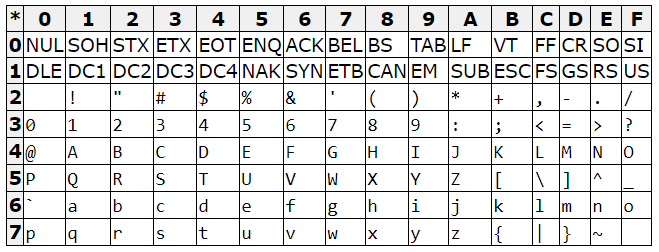
\includegraphics[width=\linewidth]{ASCII}

\easyurl{ASCII code}{http://www.cplusplus.com/doc/ascii/}
\end{frame}

\begin{frame}[fragile]{Schriftzeichen}
\begin{TPCpp}
char letter 'a';
int number = letter; // conversion
//number = 97

int number = 66;
//implicite conversion
char letter = number;
//letter = 'B'
\end{TPCpp}
\end{frame}

\note{
\begin{itemize}
\item Zeichen können in c++ mit Hochkommas geschrieben werden.
\item Die Zuweisung einer char zu einer int und umgekehrt bewirkt eine automatische / implizite Typenkonversion. Für die Konversion wird der ASCII Code verwendet.
\end{itemize}
}

\begin{frame}{Schriftzeichen}
\begin{block}{Das Alphabet}
\begin{align*}
(65)&-&10\ 00001&=&'A'\\
(66)&-&10\ 00010&=&'B'\\
&&\vdots&&\\
(97)&-&11\ 00001&=&'a'\\
(98)&-&11\ 00010&=&'b'
\end{align*}
\end{block}
\end{frame}

\note{
\begin{itemize}
\item Die Zeichen des Alphabets sind im ASCII Code so positioniert, dass durch Weglassen der ersten 2 bits direkt die Position des Buchstabens im Alphabet errechnet werden kann.
\end{itemize}
}

\begin{frame}[fragile]{string: C-style Character String}
\begin{TPCpp}
//initialisation with string literal
char text = "bool";
//equivalent to:
char text = {'b','o','o','l','\0'};
\end{TPCpp}

\begin{block}{Weaknesses}
\begin{itemize}
\item Konstante Länge (ist ein Array)
\item Ist für die meisten Operatoren nicht überladen.
\item Kennt die eigene Länge nicht.
\end{itemize}
\end{block}
\end{frame}

\begin{frame}[fragile]{string}
\begin{TPCpp}
#include <string>
std::string text1 = "bool";
//A string knows its length
text1.length();

//initialize with variable length n
//and fill with 'a'
std:string text2 (n, 'a');
//string understands comparisons
//and many other operations
text1 == text2; 
\end{TPCpp}

\easyurl{More information on strings}{http://www.cplusplus.com/reference/string/string/}
\end{frame}
%TODO extend info on string?

\note{\begin{itemize}
\item Spezialisierte Klasse die Zeichenreihen
speichern kann.
\item Grosser Funktionsumfang
\end{itemize}}

\title{PVK Lektion 5}

\maketitle

\begin{TFTimeSchedule}
\item 15' Verzweigungen
\item 15' Schleifen
\item 15' Übungen
\item 10' Besprechung
\end{TFTimeSchedule}

\begin{frame}[fragile]{Verzweigungen: if ... else}
\begin{TFCpp}
if (condition)
	statement1;
else{
	statement2;
	statement3;
}
\end{TFCpp}
\end{frame}

\begin{frame}[fragile]{Verzweigungen: switch}
\begin{TPCpp}
switch (var) {
	case 1: cout<<"one"<<endl;
	anotherStatement;
	break;
	
	case 2: cout<<"two"<<endl;
	case 3: cout<<"three"<<endl;
	break;
	
	case 4: cout<<"four"<<endl;
	break;
	
	default: cout<<"default"<<endl;
}
\end{TPCpp}
\end{frame}

\note{\begin{itemize}
\item var wird auf bestimmte Ganzzahl-Zustaende
ueberprueft. Fuer jeden case koennen statements
ausgefuehrt werden.
\item Das sukzessive ausfuehren von cases, nach
einem Match wird nur von einem break unterbrochen.
\item Der default case wird ausgefuehrt, falls 
vorher kein Match passiert ist, oder falls nach
einem Match kein break ausgefuehrt wurde.
\end{itemize}}

\begin{frame}{Schleifen: Welche Schleife in welchen Fall?}
\begin{block}{Motivation}
\begin{itemize}
\item So wenig code wie möglich.
\item Einfach lesbarer code.
\end{itemize}
\end{block}
\begin{block}{Möglichkeiten}
\begin{itemize}
\item \textbf{for}: Es wird ein Zähler benötigt, Zähler wird nach der Schleife nicht mehr benötigt.

\emph{Wiederhole ein statement $n$ mal.}
\item \textbf{while}: Die Bedingung hängt von einer Variable ab, die bereits vor der Schleife existiert.

\emph{Dekrementiere $x$ bis es ein Vielfaches von 5 ist.}
\item \textbf{do}: Die Bedingung hängt von einer Variable ab, die erst in der Schleife erhalten wird.

\emph{Führe $cin>>x$ aus bis $x>3$}
\end{itemize}
\end{block}
\end{frame}

\begin{frame}[fragile]{Schleifen: while}
\begin{TPCpp}
while(condition)
	statement;
	
while(condition){
	statement1;
	statement2;
}
\end{TPCpp}

\begin{block}{Wichtig}
\begin{itemize}
\item Bedingung, Veränderung, Terminierung!
\item Eine leere Bedingung wird nicht kompiliert!
\end{itemize}
\end{block}
\end{frame}

\note{\begin{itemize}
\item Eine Schleife muss immer so geschrieben sein,
dass durch eine Veraenderung die gesetze Bedingung
zwingend erreicht wird und somit das Programm
terminiert.
\item Diese drei Elemente sind in der for Schleife
einfach zu implementieren (naechste Folie)
\end{itemize}}

\begin{frame}[fragile]{Schleifen: for}
\begin{TPCpp}
for(int i = 0; i<10; i = i+2){
	statement1;
	statement2;
}


for(;not_done;){
	statement1;
}
\end{TPCpp}

\begin{block}{Wichtig}
\begin{itemize}
\item Der Ausdruck (i = i+2) wird erst nach den statements ausgeführt!
\item Eine leere Bedingung entspricht true!
\end{itemize}
\end{block}

\end{frame}

\begin{frame}[fragile]{Schleifen: do while}
\begin{TPCpp}
do{
	statement1;
	statement2;
}
while(condition);
\end{TPCpp}
\end{frame}

\title{PVK Lektion 6}

\maketitle

\begin{TFTimeSchedule}
\item 15' Funktionen
\item 5' Gültigkeitsbereich
\item 10' Überladungen
\item 15' Übungen
\item 10' Besprechung
\end{TFTimeSchedule}

\begin{frame}[fragile]{Funktionen: Struktur}
\begin{TPCpp}
<r_type> <function_name> (<ptype> <pname>)
{
	// Koerper / Funktionsdefinition
}
\end{TPCpp}

\begin{block}{Struktur}
\begin{itemize}
\item Rückgabetyp
\item Funktionsname
\item Funktionsparameter / Funktionsargumente
\item Funktionskörper
\end{itemize}
\end{block}
\end{frame}

\note{\begin{itemize}
\item Ein Rueckgabetyp der nicht void ist verlangt
nach einem return statement des entsprechenden Typs
im Funktionskoerper.
\end{itemize}}

\begin{frame}[fragile]{Funktionsdefinition und -deklaration}
\begin{TFCpp}
void g (...); //Deklaration von g

void f (...)
{
	g(...);
}

void g (...) // Definition von g
{
	f(...);
}
\end{TFCpp}
\end{frame}

\note{\begin{itemize}
\item Die Deklaration einer Funktion muss vor ihrem 
ersten Aufruf passieren.
\item Die Definition einer Funktion kann spaeter erfolgen,
muss aber definitiv vorhanden sein, falls die Funktion
aufgerufen wird. Das heisst, die Definition wird erst 
nachgeschlagen, wenn ein Aufruf stattfindet.
\item Es darf keine Funktionsdefinition in einem anderen
Funktionskoerper stattfinden.
\end{itemize}}

\begin{frame}[fragile]{Funktionen: Argumentübergabe}
\begin{TPCpp}
void change(int a){
	a = 4;
}

void change_ref(int & a){
	a = 4;
}
\end{TPCpp}

\begin{TPCpp}
int main(){
	int b = 3;
	change(b); //kein effekt
	change_ref(b); //b = 4;
}
\end{TPCpp}
\end{frame}

\note{\begin{itemize}
\item change ist ein Call by value und hat keinen Effekt,
da die Variable als Kopie uebergeben wird und somit 
Veraenderungen in der Funktion keinen Einfluss auf Variablen
ausserhalb der Funktion haben.
\item change\_ref erhaelt beim Aufruf eine Referenz auf
das Argument und kann es somit veraendern.
\item Das Einzige das sich beim Aufruf von change\_ref
unterscheidet ist, dass das Argument immer ein Lvalue
sein muss!
\end{itemize}}

\begin{frame}[fragile]{Funktionen: Call by Reference}
\begin{TPCpp}
void change_ref(int & a){
	a = 4;
}

void change_poi(int * a){
	*a = 4;
}
\end{TPCpp}

\begin{TPCpp}
int main(){
	int b = 3;
	change_poi(&b); //b = 4;
}
\end{TPCpp}
\end{frame}

\note{\begin{itemize}
\item Beim Call by reference mit pointern muss ein
Pointer auf das Argument uebergeben werden, der dann im
Funktionskoerper dereferenziert wird.
\item Beim Aufruf von change\_poi muss eine Adresse/ 
ein Pointer uebergeben werden!
\end{itemize}}

\begin{frame}[fragile]{Funktionen: Return by Reference}
\begin{TPCpp}
int & increment ( int & i){
	i = i + 1;
	return i;
}
\end{TPCpp}

\begin{TPCpp}
int main(){
	int i = 3;
	increment(increment(i));
	++(++i));
}
\end{TPCpp}
\end{frame}

\note{\begin{itemize}
\item Damit die Rueckgabe einer Referenz moeglich ist, muss
das Argument als Referenz uebergeben worden sein.
\item Die Rueckgabe einer Referenz ermoeglich das Verketten
von Funktionen.
\end{itemize}}

\begin{frame}[fragile]{Funktionen: Rekursion}
\begin{TPCpp}
void f(){
	f(); //Endlosaufruf
}
\end{TPCpp}
\end{frame}

\begin{frame}[fragile]{Funktionen: Rekursion}
\begin{TPCpp}
// POST: return value n!
unsigned int fac (unsigned int n)
{
	//Abbruchbedingung
	if (n <= 1) return 1;
	
	//Rekursiver Aufruf
	return n* fac(n-1);
}
\end{TPCpp}
\end{frame}

\note{\begin{itemize}
\item Eine rekursive Funktion besteht immer aus einer Abbruch-
bedingung und einem rekursiven Aufruf.
\item Vorteile: Einfacher und Verstaendlicher Code
\item Nachteile: Stack overflow moeglich, langsameres
Debugging sehr viel schwieriger.
\end{itemize}}

\begin{frame}{Gültigkeitsbereich}
\begin{block}{Bereiche}
\begin{enumerate}
\item In einer Funktion oder in einem Block (lokale Variablen)
\item Als Parameter einer Funktion (formaler Parameter)
\item Ausserhalb aller Funktionen (globale Variablen)
\end{enumerate}
\end{block}
\begin{block}{Regel}
\textbf{Es wird immer die nähere Definition genutzt!}
\end{block}
\end{frame}

\begin{frame}[fragile]{Gültigkeitsbereich}
%\begin{TPCpp}
%for (int i = 0; i<10; i++) cout<<i<<endl;
%//cout<<i<<endl; //not possible
%\end{TPCpp}
\small
\begin{TPCpp}
int i = 2; //Globale Variable

void fun(){cout<<i;}

int main(){
	int i = 5;
	{ //Block
		int i = 3;
		cout<<i;
	}
	cout<<i;
	fun();
}
\end{TPCpp}
\normalsize

\begin{block}{Regel}
\textbf{Es wird immer die nähere Definition genutzt!}
\end{block}
\end{frame}

\begin{frame}[fragile]{Überladungen: Funktionen}
\begin{TFCpp}
void print_variable(int a){
	cout<<"This is an int."<<endl;
}

void print_variable(double a){
	cout<<"This is a double."<<endl;
}

int print_variable(int a, int b){
	cout<<"Two ints."<<endl;
	return 2;
}
\end{TFCpp}
\end{frame}

\note{\begin{itemize}
\item Funktionsueberladung funktioniert mit Unterscheidung
durch Anzahl Argumente und durch Typ der Argumente.
\item Funktionsueberladung funktioniert weder mit Unterscheidung
durch Rueckgabetyp noch durch Variablennamen.
\item Ueberladungen dürfen andere Rueckgabetypen haben!
\end{itemize}}

\begin{frame}[fragile]{Überladungen: Operatoren}
\begin{block}{Motivation}
\begin{itemize}
\item Operatoren sind nur für primitive Datentypen definiert.
\item Operatoren sind einfacher zu benutzen als Funktionen.
\item \textbf{Neudefinition für jeden neuen Datentyp!}
\end{itemize}
\end{block}

\begin{TPCpp}
<r_type> operator<target_op> (<ptype> <pname>)
{
	//Koerper / Funktionsdefinition
}
\end{TPCpp}
\end{frame}

\begin{frame}[fragile]{Überladungen: Operatoren}
\begin{TPCpp}
class rational {
	int n,d;
	public:
	rational& operator+= (const rational b);	
};
\end{TPCpp}

\vfill

\[\frac{a_n}{a_d} \leftarrow \frac{a_n}{a_d}+\frac{b_n}{b_d} = \frac{a_n\cdot b_d}{a_d\cdot b_d}+\frac{b_n\cdot a_d}{b_d\cdot a_d}\]
\end{frame}

\note{\begin{itemize}
\item Neuer Datentyp: rational
\item Wir moechten die Addition per operator ermoeglichen
\item Dazu definieren wir zuerst die Mitgliedsfunktion +=
\item Folgend definieren wir basierend auf += den operator+
\item So muessen wir bei einer Aenderung der Struktur nur
+= anpassen und + stimmt auch.
\end{itemize}}

\begin{frame}[fragile,label=POperatorOverloading]{Überladungen: Operatoren}
\begin{TPCpp}
rational& rational::operator+=(const rational b){
	this->n = this->n*b.d + this->d*b.n;
	this->d = this->d*b.d;
	return *this;
}

rational operator+ (const rational& a, const rational& b){
	rational temp = {0,1};
	temp += a;
	temp += b;
	return temp;
}
\end{TPCpp}

\hyperlink{BOverloadableOperators}{\beamergotobutton{Overloadable Operators}} \hyperlink{BHowToOverload}{\beamergotobutton{Wie überladen?}}
\end{frame}

\note{\begin{itemize}
\item Funktionstyp per Konvention: Zuweisungsoperatoren geben eine
Referenz zurueck! Somit ist eine Verkettung von Zuweisungen moeglich.
\item Funktionsname: Schluesselwort operator und danach der Operator.
\item Funktionsargumente: Binaerer Operator, hat 2 Argumente:
Dasjenige auf der linken Seite und dasjenige auf der rechten Seite.
Sie werden in dieser Reihenfolge ueberreicht.
\item += als Mitglied, + als normale Funktion
\end{itemize}}

\title{PVK Lektion 7}

\maketitle

\begin{TFTimeSchedule}
\item 20' Stellenwertsysteme
\item 10' EBNF
\item 15' Übungen
\item 10' Besprechung
\end{TFTimeSchedule}

\begin{TFTwoColumns}[Stellenwertsysteme: Binäre Darstellung]{
\begin{align*}
91310&=\uncover<2-5>{10*9131+&0}\\
\uncover<3-5>{9131&=10*913+&1}\\
\uncover<4-5>{913&=10*91+&3\\
91&=10*9+&1\\
9&=10*0+&9}
\end{align*}
}
{
\begin{align*}
\uncover<5>{61&=2*30+&1\\
30&=2*15+&0\\
15&=2*7+&1\\
7&=2*3+&1\\
3&=2*1+&1\\
1&=2*0+&1}
\end{align*}
}
\end{TFTwoColumns}

\begin{frame}{Stellenwertsysteme: Binäre Darstellung}
\begin{tabular}{lllllll}
&&&&&&$\sum$\\
Ziffern&9&1&3&1&0\\
Multiplikator&\uncover<2-4>{10000&1000&100&10&1}\\
Wert&\uncover<3-4>{90000&1000&300&10&0&91310}
\end{tabular}

\vfill

\begin{tabular}{llllllll}
\uncover<4>{&&&&&&&$\sum$\\
Ziffern&1&1&1&1&0&1\\
Multiplikator&32&16&8&4&2&1\\
Wert&32&16&8&4&0&1&61\\}
\end{tabular}
\end{frame}

\begin{frame}{Stellenwertsysteme: Negative Binärzahlen}
\begin{center}
\begin{tabular}{rrrrrr}
bin&uint&int&bin&uint&int\\\midrule
0000&0&0&1000&8&-8\\
0001&1&1&1001&9&-7\\
0010&2&2&1010&10&-6\\
0011&3&3&1011&11&-5\\
0100&4&4&1100&12&-4\\
0101&5&5&1101&13&-3\\
0110&6&6&1110&14&-2\\
0111&7&7&1111&15&-1
\end{tabular}
\end{center}
\end{frame}

\note{\begin{itemize}
\item Negative Zahlen im Binärsystem werden im Zweierkomplement
abgespeichert.
\item Das bedeutet, dass das erste Bit negativ bewertet wird.
\end{itemize}}

\begin{frame}{Stellenwertsysteme: Dezimalzahlen im Binärsystem}
\begin{center}
\begin{tabular}{llllllllll}
&&&&&&&&&$\sum$\\
digit:&1&1&0&1&.&1&0&1\\
factor:&8&4&2&1&&$\frac{1}{2}$&$\frac{1}{4}$&$\frac{1}{8}$\\
value&8&4&0&1&&$\frac{1}{2}$&0&$\frac{1}{8}$&13.625
\end{tabular}
\end{center}
\end{frame}

\begin{TFTwoColumns}[Stellenwertsysteme: Dezimalzahlen im Binärsystem]
{
\begin{center}
\begin{tabular}{l|l|l}
$x$&$d_i$&$x-d_i$\\\hline
1.934&1&0.934\\
\uncover<2->{9.34&9&0.34\\}
\uncover<3->{3.4&3&0.4\\
4&4&0}
\end{tabular}
\end{center}
}
{
\begin{center}
\uncover<4->{
\begin{tabular}{r|l|l}
$x$&$b_i$&$x-b_i$\\\hline
1.9&1&0.9\\
\uncover<5->{1.8&1&0.8\\}
\uncover<6->{\textbf{1.6}&1&0.6\\}
\uncover<7->{1.2&1&0.2\\}
\uncover<8->{0.4&0&0.8\\}
\uncover<9->{\textbf{1.6}&1&0.6\\}
\uncover<10->{&$\vdots$&}
\end{tabular}}
\end{center}
\uncover<11->{\begin{equation*}
1.1\overline{1100}
\end{equation*}}
}
\end{TFTwoColumns}

\note{
\begin{itemize}
\item Erklärung im Dezimalsystem
\begin{enumerate}
\item Stelle abziehen.
\item Verschiebung mit mal 10.
\end{enumerate}
\item Erklärung im Binärsystem
\begin{enumerate}
\item Stelle abziehen.
\item Verschiebung mit mal 2.
\end{enumerate}
\item Zusatzinfo: Es git also Zahlen, die in bestimmten Zahlensystemen keine \textbf{finite Darstellung} haben!
\end{itemize}
}

\begin{frame}{Stellenwertsysteme: Unser kleines 10bit Fliesskommasystem}
\begin{block}{Beschreibung von Fliesskommasystemen}
$\mathcal{F}(\underbrace{\beta}_\text{Basis $\geq$ 2},\overbrace{p}^\text{Anzahl Stellen$\geq$1},\underbrace{e_{min},e_{max}}_\text{Kleinster und Grösster Exponent})$
\end{block}
\end{frame}

%TODO check presentation length - change if time overflow

\begin{frame}{$\mathcal{F}(2,6,0,15)$}
\begin{Huge}
\[{\color{red}{0}}{\color{green}{0000}}{\color{blue}{00000}}\]
\end{Huge}
\begin{itemize}
\item\textcolor{red}{Vorkommastelle}
\item\textcolor{blue}{Nachkommastellen}
\item\textcolor{green}{Exponent}
\end{itemize}
\begin{block}{Beispiele}
$\underbrace{\textcolor{red}{1}.\textcolor{blue}{11111}\cdot 2^{\textcolor{green}{15}}}_\text{Grösste Zahl}\qquad\qquad\underbrace{\textcolor{red}{0}.\textcolor{blue}{00001}\cdot 2^{\textcolor{green}{0}}}_\text{Kleinste Zahl}$
\end{block}
\end{frame}

\note{\begin{itemize}
\item Wir möchten auch negative Exponenten.
\item Interpretation als unsigned int mit Verschiebung ins negative (IEEE 754 Standard), schnellere Rechnungen möglich)
\item 
\end{itemize}}

\begin{frame}{$\mathcal{F}(2,6,-8,7)$}
\begin{Huge}
\[{\color{red}{0}}{\color{green}{0000}}{\color{blue}{00000}}\]
\end{Huge}
\begin{itemize}
\item\textcolor{red}{Vorkommastelle}
\item\textcolor{blue}{Nachkommastellen}
\item\textcolor{green}{Exponent}
\end{itemize}
\begin{block}{Beispiele}
$\underbrace{\textcolor{red}{1}.\textcolor{blue}{11111}\cdot 2^{\textcolor{green}{7}}}_\text{Grösste Zahl}\qquad\qquad\underbrace{\textcolor{red}{0}.\textcolor{blue}{00001}\cdot 2^{\textcolor{green}{-8}}}_\text{Kleinste Zahl}$
\end{block}
\end{frame}

\note{
\begin{itemize}
\item Wir brauchen negative Zahlen!
\item Wir brauchen das erste Bit nicht zwingend wenn wir annehmen, dass es immer 1 ist.
\end{itemize}
}

\begin{frame}{Stellenwertsysteme: $\mathcal{F}^\ast(2,6,-8,7)$}
\begin{Huge}
\[{\color{red}{0}}{\color{green}{0000}}{\color{blue}{00000}}\]
\end{Huge}
\begin{itemize}
\item\textcolor{red}{Vorzeichenstelle}
\item\textcolor{blue}{Nachkommastellen}
\item\textcolor{green}{Exponent}
\end{itemize}
\begin{block}{Beispiele}

$\underbrace{\textcolor{red}{+}1.\textcolor{blue}{11111}\cdot 2^{\textcolor{green}{7}}}_\text{Grösste Zahl}\qquad\qquad \underbrace{\textcolor{red}{-}1.\textcolor{blue}{11111}\cdot2^{\textcolor{green}{7}}}_\text{Kleinste Zahl}\qquad\qquad\underbrace{\textcolor{red}{+}1.\textcolor{blue}{00000}\cdot2^{\textcolor{green}{-8}}}_\text{Kleinste positive Zahl}$

\end{block}
\end{frame}

\note{\begin{itemize}
\item Wir können 0 nicht mehr darstellen
\item Ein Exponent für spezielle Zahlen: -8 = 0000
\item Und die Nachkommastellen als Codierung für diese Zahlen
\end{itemize}
}
\begin{frame}{$\mathcal{F}^\ast(2,6,-7,7)$}
\begin{Huge}
\[{\color{red}{0}}{\color{green}{0000}}{\color{blue}{00000}}\]
\end{Huge}
\begin{itemize}
\item\textcolor{red}{Vorzeichenstelle}
\item\textcolor{blue}{Nachkommastellen}
\item\textcolor{green}{Exponent}
\end{itemize}
\begin{block}{Beispiele}
\begin{center}
$\underbrace{\textcolor{red}{0}\textcolor{green}{0000}\textcolor{blue}{00000}}_\text{Null}\qquad \underbrace{\textcolor{red}{0}\textcolor{green}{0000}\textcolor{blue}{00001}}_{+\infty}\qquad\underbrace{\textcolor{red}{0}\textcolor{green}{0000}\textcolor{blue}{00010}}_{-\infty}\qquad\underbrace{\textcolor{red}{0}\textcolor{green}{0000}\textcolor{blue}{00011}}_\text{NaN}$
\end{center}
\end{block}
\end{frame}

\note{
\begin{itemize}
\item Wir können 0 nicht mehr darstellen
\item Ein Exponent für spezielle Zahlen: -8 = 0000
\item Und die Nachkommastellen als Codierung für diese Zahlen
\item Jetzt verstehen wir auch 32bit float und 64bit double
\end{itemize}
}

\begin{frame}[fragile]{Tipps zu Fliesskommazahlen}
\begin{TFCpp}
//Kein Vergleich gerundeter Zahlen
double  a = 1.1; 
if(100*a == 110) cout<<true<<endl;

//Keine Add. versch. grosser Zahlen
float a = 67108864.0f + 1.0f 
//output: 67108864

//Keine Subtr. aehnlich grosser Zahlen
float x_0 = 0.2; 
//represented as: 0.20000000298
float x_1 = 6*x_0 - 1; //is not 0.2
\end{TFCpp}
\end{frame}

\begin{frame}[fragile]{Backus-Naur-Form}
\begin{block}{Kurz und simpel}
\textbf{Die Backus-Naur-Form ist eine Sprache die mit einfacher Syntax beschreibt, welche Sätze mit den Wörtern einer Sprache gebildet werden dürfen.}
\end{block}
\begin{block}{Aufbau}
\begin{itemize}
\item Alphabet = Terminalsymbole
\item Satzbau = Produktionsregeln = Nichtterminalsymbol
\end{itemize}
\end{block}

\begin{TPPython}
ZifferAusserNull = "1" | "2" | "3" | "4" | "5" | "6" | "7" | "8" | "9" ;
Ziffer = "0" | ZifferAusserNull ;
\end{TPPython}
\end{frame}

\begin{frame}[fragile]{Erweiterte Backus-Naur-Form: Beispiel}
\begin{TFPython}
ZifAussNull = "1" | "2" | "3" | "4" | "5" | "6" | "7" | "8" | "9" ;
Zif = "0" | ZifAussNull ;

Zwoelf = "1", "2" ;
Dreihundertzwoelf = "3", Zwoelf ;

NatZahl = ZifAussNull, { Zif } ;
GanzeZahl = "0" | [ "-" ], NatZahl ;
\end{TFPython}
\end{frame}

\begin{frame}[fragile]{Vorteile der EBNF}
\begin{TPPython}
seq = term | term "_" seq
term = "A" | "A" lowerterm | lowerterm
lowerterm = "a" | "a" lowerterm


seq = term | term "_" seq
term = "A" { "a" } | "a" { "a" }

seq = term [ "_" seq ]
term = "A" { "a" } | "a" { "a" }
\end{TPPython}
\end{frame}

\note{\begin{itemize}
\item Die erweiterte BNF fuehrt zusaetzlich 
geschweifte Klammern ein. Diese bedeuten eine
beliebige Anzahl Wiederholungen des enthaltenen
Elements.
\item Weiterhin werden eckige Klammer eingefuehrt.
Diese bedeuten, dass der Inhalt 0 oder 1 mal
eingefügt werden kann. Somit ist das eine Alternative.
\end{itemize}}

\title{PVK Lektion 8}

\maketitle

\begin{TFTimeSchedule}
\item 15' Klassen
\item 15' Dynamische Datenstrukturen
\item 15' Übungen
\item 10' Besprechung
\end{TFTimeSchedule}

\begin{frame}{Klassen: Motivation}
\begin{block}{Was}
\begin{itemize}
\item Klassen: Kombination von Variablen und Funktionen
\item Instanzen
\item Objekte
\end{itemize}
\end{block}

\begin{block}{Objektorientiertes Programmieren}
Die Grundidee besteht darin, die Architektur einer Software an den Grundstrukturen desjenigen Bereichs der Wirklichkeit auszurichten, der die gegebene Anwendung betrifft.
\end{block}

\begin{block}{Wieso}
\begin{itemize}
\item Verkapselung
\item Wiederverwendbarkeit
\end{itemize}
\end{block}

\easyurl{Objektorientiertes Programmieren}{https://de.wikipedia.org/wiki/Objektorientierte_Programmierung}
\end{frame}

\begin{frame}[fragile]{Klassen: Grundlagen}
\begin{block}{Mitglieder}
\begin{itemize}
\item \textbf{Mitgliedsfunktion}:

Funktion die in der Klasse angelegt wird.
\item \textbf{Mitgliedsvariable}: 

Variable die in der Klasse angelegt wird.
\end{itemize}

Mitglieder können nur über eine Instanz der Klasse aufgerufen werden. 
\end{block}

\begin{TPCpp}
//Definition der Klasse
class Vector {...}; 
Vector v1; //Deklaration einer Instanz
v1.memberVariable;
v1.memberFunction();
Vector* pv1 = &v1;
pv1->memberVariable;
\end{TPCpp}
\end{frame}

\note{\begin{itemize}
\item Zugriff auf Mitglieder ueber eine Instanz der
Klasse funktioniert mit dem Punktoperator.
\item Zugriff auf Mitglieder ueber einen Pointer
auf eine Instanz funktioniert mit dem Pfeiloperator.
Dieser ist gleichwertig mit *(pointer).member.
\end{itemize}}

\begin{frame}[fragile]{Klassen: Grundlagen}
\begin{block}{Verkapselung}
\begin{itemize}
\item \textbf{Private Mitglieder}:

Nach dem Schlüsselwort \verb+private+ kommen alle Variablen die versteckt sein sollen.
\item \textbf{Öffentliche Mitglieder}:

Nach dem Schlüsselwort \verb+public+ kommen alle Variablen die öffenlich sein sollen.
\end{itemize}

Nur öffenlichte Mitglieder können über einen der beiden Zugriffsoperatoren erreicht werden. 

\vspace{3ex}

Mitgliedsfunktionen haben Zugriff auf private Migliedsvariablen.
\end{block}
\end{frame}

\begin{frame}[fragile]{Klassen: Grundlagen}
\begin{TFCpp}
class Vector {
private:
	double x;
	double y;
};
\end{TFCpp}

\null\vfill\null

\easyurl{Codeboard}{https://codeboard.io/projects/82028}$\hfill$\easyurl{Zusätzliches Beispiel}{https://codeboard.io/projects/81739}
\end{frame}

\begin{frame}[fragile]{Klassen: Konstruktoren}
\begin{block}{Konstruktor}
\begin{itemize}
\item Öffentliche Mitgliedsfunktion
\item Wird automatisch beim Erstellen einer Instanz der Klasse aufgerufen!
\item Wird eingesetzt um Mitgliedsvariablen zu initialisieren.
\end{itemize}
\end{block}
\begin{TPCpp}
public: 
	Vector (){
		x = 0;
		y = 0;
	}
	Vector (double _x, double _y) : x(_x), y(_y) {}
\end{TPCpp}
\end{frame}

\note{\begin{itemize}
\item Der Konstruktor ist eine Funktion mit dem Namen der Klasse.
\item Der default-Konstruktor, der keine Argumente uebernimmt wird aufgerufen, wenn eine Instanz der Klasse erzeugt wird und keine Argumente uebergeben werden.
\item Der nicht-default-Konstruktor mit 2 Argumenten ist eine Ueberladung des default-Konstruktors.
\item Die Initialisierungsliste wird benutzt um Mitgliedsvariablen 
zu initialisieren. Sie ist hier nicht strikt notwending,
wird aber gebraucht sobald eine Klasse konstante
Mitgliedsvariablen hat, denn diese koennen nur so
initialisiert werden.
\end{itemize}}

\begin{frame}[fragile]{Klassen: Konstruktoren}
\begin{TFCpp}
class Vector {
	double x;
	double y;
public:
	Vector () : x(0),y(0){}
	Vector (double _x, double _y) 
		: x(_x),y(_y) {}
};

Vector v1;
Vector v2();
Vector v3(1.0, 2.3);
\end{TFCpp}
\end{frame}

\note{\begin{itemize}
\item Mitglieder ohne spezifizierung sind automatisch privat!
\item Der Konstruktor wird auch ohne Klammern aufgerufen.
\item Der Konstruktor folgt immer dem Schema
$<$Klassenname$>$ ($<$argumente$>$) $<$initialisierungsliste$>$
$\{<$aktionen$>\}$
\item Der Konstruktor hat immer den Rueckgabetyp void.
Das wird nicht extra angegeben sondern ist so bereits
vorgemerkt.
\end{itemize}}

\begin{frame}[fragile]{Klassen: Zugriffsmethoden}
\begin{block}{Zugriff}
\begin{itemize}
\item Der Zugriff ist durch Verkapselung eingeschränkt.
\item Lösung: Sicherer Zugriff mit Zugriffsmethoden.
\end{itemize}
\end{block}

\vfill

\begin{TPCpp}
double get_x() const {return x;}
double get_y() const {return y;}

void set_x(const double _x) {x = _x;}
void set_y(const double _y) {y = _y;}
\end{TPCpp}
\end{frame}

\note{\begin{itemize}
\item Konstante Mitgliedsfunktionen koennen
Mitgliedsvariablen nicht verändern (ausser diese sind
mutable).
\end{itemize}}

\begin{frame}[fragile]{Klassen: Zugriff auf Mitglieder}
\begin{block}{this}
\begin{itemize}
\item Der \verb+this+ Pointer speichert die Adresse seiner Instanz einer Klasse.
\item Er ist in jeder Klasse vorhanden und kann in Mitgliedsfunktionen benutzt werden um auf die aktuelle Instanz zuzugreifen.
\end{itemize}
\end{block}

\vfill

\begin{TPCpp}
double get_x() const {return this->x;}
double get_y() const {return (*this).y;}
\end{TPCpp}

\end{frame}

\begin{frame}[fragile]{Klassen: Arithmetische Operatoren}
\begin{block}{Argumentübergabe}
\begin{itemize}
\item Die Operatoren, die als Mitgliedsfunktion überladen werden, erhalten die aufrufende Instanz als erstes Argument.
\item Der Rückgabetyp hängt vom überladenen Operator ab. Für Zuweisungen wird eine Referenz zurückgegeben.
\end{itemize}
\end{block}

\begin{TPCpp}
Vector& operator+= (const Vector& b){
    x += b.get_x();
    y += b.get_y();
    return *this;
}
//Im main:
Vector v3(3,4),v4(1,2);
v3 += v4;
\end{TPCpp}
\end{frame}

\begin{frame}[fragile]{Klassen: Arithmetische Operatoren}
\begin{TFCpp}
Vector& operator+= (const Vector& b){
    x += b.get_x();
    y += b.get_y();
    return *this;
}

//Ausserhalb der Klasse
Vector operator+ (const Vector& a, const Vector& b) {
	Vector res = a;
	res += b;
	return res;
}
\end{TFCpp}

\end{frame}

\note{\begin{itemize}
\item Wenn die Ueberladung des += operators ausserhalb
der Klasse stattfindet erlaubt er implizite Typen-
konversion. Ansonten muesste er immer ueber eine
Instanz der Klasse aufgerufen werden.
\end{itemize}}

\begin{frame}[fragile]{Dynamische Datentypen - Stack}
\begin{TFCpp}
class stack {
public:
	void push (int value){...}
	int pop (){}
	...
	void print (){...}
	
private:
	ln* top_node; //ln = list node
};

struct ln {
	int key;
	ln * next;
}
\end{TFCpp}
\end{frame}

\begin{frame}[fragile]{Dynamische Datentypen - Stack}
\begin{TPCpp}
stack s1;
s1.push(1);
s1.push(2);
s1.push(3);
s2(s1);
\end{TPCpp}

\begin{center}
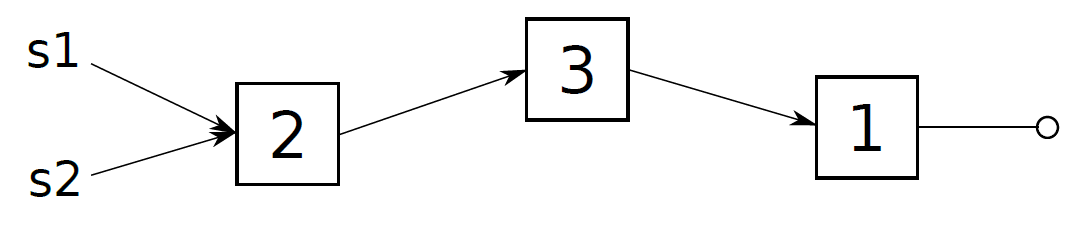
\includegraphics[width=0.9\linewidth]{Pictures/Stack1}
\end{center}

\end{frame}

\note{\begin{itemize}
\item Mit dem Standard Kopierkonstruktor werden einfach
die Mitgliedsvariablen der Struktur kopiert. In
diesem Fall also ein Pointer auf das erste Element
des Stacks.
\item Da wird gerne eine sogenannte tiefe Kopie
haben moechten reicht uns das nicht.
\end{itemize}}

\begin{frame}[fragile]{Dynamische Datentypen - Stack - Tiefe Kopie}
\begin{TFCpp}
stack::stack(const stack& s) : top_node(0) {
	copy(s.top_node, top_node);
}

void stack::copy(const ln* from, ln*& to){
	assert (to == 0);
	if(from != 0){
		to = new ln(from->key);
		copy(from->next, to->next);
	}
}
\end{TFCpp}

\begin{TPCpp}
s2(s1);
\end{TPCpp}

\end{frame}

\note{\begin{itemize}
\item Der Kopierkonstruktor hat als Argument eine Referenz, da die Übergabe eines einfachen Wertes bereits einen Kopiervorgang benötigen würde!
\end{itemize}}

\begin{frame}[fragile]{Dynamische Datentypen - Stack - Zuweisung}
\begin{TPCpp}
stack s2;
s2.push(4);
s2.push(9);
s2 = s1;
\end{TPCpp}


\begin{center}
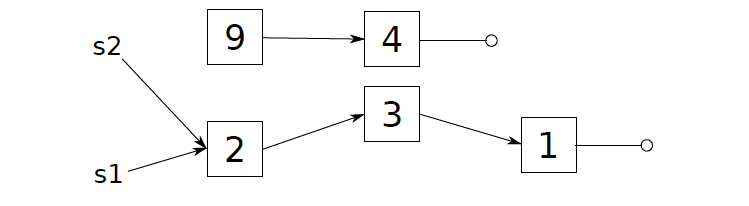
\includegraphics[width=0.9\linewidth]{Pictures/Stack2}
\end{center}
\end{frame}

\note{\begin{itemize}
\item Der Zuweisungsoperator macht immer noch eine oberflacheliche 
Kopie, setzt also nur alle Mitgliedsvariablen von s1 gleich die von s2.
\item Um das zu beheben ueberladen wir den Zuweisungsoperator.
\end{itemize}}

\begin{frame}[fragile]{Dynamische Datentypen - Stack - Zuweisung}
\begin{TFCpp}
void stack::clear(ln* from){
	if (from != 0){
		clear(from->next);
		delete from;
	}
}
\end{TFCpp}
\end{frame}

\note{\begin{itemize}
\item Bevor zugewiesen werden kann, muss der Empfaenger der Zuweisung
seinen Stack leeren. Dazu wird clear implementiert.
\end{itemize}}

\begin{frame}[fragile]{Dynamische Datenstrukturen - Stack - Zuweisung}
\begin{TPCpp}
stack& stack::operator= (const stack& s) {
	if (top_node != s.top_node) { // test for self-assignment
		clear(top_node);
		top_node = 0; // fix dangling pointer
		copy(s.top_node, top_node);
	}
return *this;
}
\end{TPCpp}

\begin{TPCpp}
s1 = s2;
\end{TPCpp}

\end{frame}

\note{\begin{itemize}
\item Vor der Ueberschreibung wird geprueft ob der 
Stack sich selbst zugewiesen wird.
\item Falls nicht wird die aufrufende Instanz
geloescht und dann mit der Kopierfunktion ueberschrieben
\item Schliesslich wird der Konvention entsprechend
eine Referenz auf die aufrufende Instanz uebergeben.
Das bewirkt weiter, dass der Zuweisungsoperator
verkettet werden kann.
\end{itemize}}

\begin{frame}[fragile]{Dynamische Datenstrukturen - Stack - Destruktor}
\begin{TFCpp}
void useStack(){
	stack temp;
	temp.push(2);
	temp.pop();
} //end of scope, destruction

stack::~stack() {
	clear(top_node);
}
\end{TFCpp}
\end{frame}

\note{\begin{itemize}
\item Beim Loeschen eines Objekts wird immer dessen
Destruktor aufgerufen. Damit im Falle einer
dynamischen Datenstruktur auch alle dynamisch
allokierten Speicherplaetze freigegeben werden
muss der Destruktor entsprechend definiert werden.
\item Daher wird die clear-Funktion fuer alle
angehaengten Nodes aufgerufen. Die uebrigen
Mitglieder der Instanz werden automatisch geloescht.
\end{itemize}}

\begin{frame}{Klassen: Spezielle Mitgliedsfunktionen}
\begin{block}{Standardmitglieder}
\begin{itemize}
\item Defaultkonstruktor
\item Kopierkonstruktor
\item Zuweisungsoperator
\item Defaultdestruktor
\end{itemize}

\end{block}

\textbf{Regel der drei:} Wenn entweder Destruktor, Kopierkonstruktor und Zuweisungsoperator neu definiert werden sollten alle drei neu definiert werden.
\end{frame}

\note{\begin{itemize}
\item Normalerweise werden diese Funktionen neu
definiert sobald eine dynamische Datenstruktur 
eingefuehrt wird, die nach der Verwaltung von
dynamisch angelegtem Speicherplatz verlangt.
Dann ist es unerlaesslich diese drei Funktionen
entsprechend auszulegen.
\end{itemize}}

\title{PVK Lektion 9}

\maketitle

\begin{TFTimeSchedule}
\item 30' Vererbung
\item 15' Übungen
\item 10' Besprechung
\end{TFTimeSchedule}

\begin{frame}[fragile]{Vererbung: Grundlagen}
\begin{TFCpp}
class A{
	... //Basisklasse
};

class B: public A{
	... //Abgeleitete Klasse
};

class C: public B{
	... 
};
\end{TFCpp}
\end{frame}

\note{\begin{itemize}
\item Vererbung erlaubt alle Mitglieder einer Basisklasse in einer
abgeleiteten Klasse zu uebernehmen und weitere hinzuzufuegen.
So kann einmal geschriebener code mehrfach verwendet werden. Weiter
kann eine ganze Familie von Klassen die ihre grundlegenden Eigenschaften
identisch Teilen. Die selben grundlegenden Eigenschaften (Basisklasse)
koennen dann auf fuer den ganzen Vererbungsbaum auf einen Schlag
angepasst werden.
\end{itemize}}

\begin{frame}[fragile]{Vererbung: Zugriffskontrolle}

\begin{tabular}{|l|lll|}
\hline
Vererbung \verb+\+ Mitglied & \verb+public+ & \verb+protected+ & \verb+private+\\\hline
\verb+public+&\verb+public+&\verb+protected+&n/a\\
\verb+protected+&\verb+protected+&\verb+protected+&n/a\\
\verb+private+&\verb+private+&\verb+private+&n/a\\\hline
\end{tabular}
\end{frame}

\begin{frame}[fragile]{Polymorphismus}
\begin{TFCpp}
class A {
	virtual void print() 
	{cout<<"A"<<endl;}
};

class B : public A {
	void print()
	{cout<<"B"<<endl;}
};

A instantce1;
instance1.print();
B instance2;
instance2.print();
A * pointer1 = &instance2;
pointer1->print();
\end{TFCpp}
\end{frame}

\note{\begin{itemize}
\item virtual bewirkt, dass die nachfolgende Methode, wenn sie in einer
Subklasse ueberschreiben wird bei Laufzeit dynamisch auswaehlt, welcher
Typ die aufrufende Instanz hat.
\item Das heisst ein Pointer der Basisklasse kann sowohl auf eine Instanz
der Basisklasse, wie auch auf eine Instanz einer davon abgleiteten Klasse
zeigen. Fuer nicht virtuelle Mitgliedsfunktionen wird dann ueber den Typ
des Pointers bestimmt welche Mitgliedsfunktion ausgefuehrt wird. Fuer
virtuelle Mitgliedsfunktionen wird dynamisch ausgewertet auf welche Instanz
der Pointer zeigt, und dann deren Version der Mitgliedsfunktion
ausgefuehrt.
\end{itemize}}

\begin{frame}{Polymorphismus und dynamische Bindung}
Ausgangspunkt: Abgeleitete Klasse die virtuelle Mitgliedsfunktion ihrere Basisklasse überschreibt.

Frage: Wann wird welche Version der Mitgliedsfunktion aufgerufen?
\begin{block}{Faustregeln}
\begin{enumerate}
\item Bei direktem Aufruf über eine Instanz wird immer die dem Typ entsprechende Mitgliedsfunktion aufgerufen.
\item Bei indirektem Aufruf über einen Pointer wird für nicht virtuelle Mitgliedsfunktionen immer die dem Typ des Pointers entsprechende Mitgliedsfunktion aufgerufen.
\item Bei indirektem Aufruf über einen Pointer wird für virtuelle Mitgliedsfunktionen immer die dem dereferenzierten Typ des Pointers entsprechende Mitgliedsfunktion aufgerufen.
\end{enumerate}
\end{block}
\end{frame}

\begin{frame}[fragile]{Abstrakte Basisklasse}
\begin{TFCpp}
class A {
	virtual void print() = 0;
};

class B : public A {
	void print()
	{cout<<"B"<<endl;}
};

//A instance1; //Forbidden
A * pointer1 = new B; //Allowed
\end{TFCpp}
\end{frame}

\note{\begin{itemize}
\item Wenn eine virtuelle Mitgliedsfunktion = 0 gesetzt wird, wird sie zur
rein virtuellen Methode und die inhabende Klasse wird zur abstrakten
Basisklasse.
\item Das heisst, das die Klasse nicht mehr instantiiert werden kann,
sondern nur als Basis fuer abgeleitete Klassen fungiert.
\end{itemize}}

\begin{frame}[fragile]{Konstruktoren}
\begin{TFCpp}
class A {
	int a;
public:
	A(int _a) : a(_a){}
};

class B : public A {
	int b;
public:
	B(int _a, int _b) : A(_a), b(_b) {}
};
\end{TFCpp}
\end{frame}

\note{\begin{itemize}
\item Da die privaten Mitgliedsvariablen der Basisklasse fuer die 
abgeleiteten Klassen nicht mehr verfuegbar sind, muss im Konstruktor
der abgeleiteten Klasse der Konstruktor der Basisklasse aufgerufen werden.
\end{itemize}}

\begin{frame}[fragile]{is a - has a}
\begin{TFCpp}
class point {
public:
	double x;
	double y;
};

class circle : private point {
private:
	double radius;
};
\end{TFCpp}
\end{frame}

\note{\begin{itemize}
\item Die Klasse circle erbt von der Klasse Punkt und
\textbf{ist} somit ein Punkt.
\item Dies ist die erste Moeglichkeit der Implementation einer Kreis Klasse die Zugriff auf die
Variablen eines Punkts hat.
\end{itemize}}

\begin{frame}[fragile]{is a - has a}
\begin{TFCpp}
class point {
public:
	double x;
	double y;
};

class circle {
private:
	double radius;
	point p;
};
\end{TFCpp}
\end{frame}

\note{\begin{itemize}
\item Die Klasse circle erbt nicht von point sondern 
\textbf{hat} einen Punkt als Mitglied.
\item Der Unterschied beider Implementierungen ist
minimal, eigentlich unterscheidet sich nur der
Zugriff auf die Mitgliedsvariablen des Punkts.
\item Sprachlich unterscheidet man von Fall 1 
\textbf{``ist''} zu Fall 2 \textbf{``hat''} einen
Punkt.
\end{itemize}}

\begin{frame}[fragile]{is a - has a}
\begin{TFCpp}
class University {
private:
	std::vector<Student> students_;
};

class Student {
private:
	Legi legi_;
};

class Phys_Student : public Student {};

class Legi {
	int immatriculation_year_;
};
\end{TFCpp}
\end{frame}

\title{Backup Slides}

\maketitle

\begin{frame}[fragile,label=BOverloadableOperators]{Überladungen: Operatoren}
\begin{PTable}{*{6}{p{0.1\linewidth}}}
\verb-+-&\verb+-+&\verb+*+&\verb+/+&\verb+%+&\cellcolor{red!25}\verb+^+\\\hline
\verb+&+&\cellcolor{red!25}\verb+|+&\cellcolor{red!25}\verb+~+&\verb+!+&\verb+,+&\verb+=+\\\hline
\verb+<+&\verb+>+&\verb+<=+&\verb+>=+&\verb-++-&\verb+--+\\\hline
\verb+<<+&\verb+>>+&\verb+==+&\verb+!=+&\verb+&&+&\verb+||+\\\hline
\verb-+=-&\verb+-=+&\verb+/=+&\verb+%=+&\cellcolor{red!25}\verb+^=+&\cellcolor{red!25}\verb+&=+\\\hline
\cellcolor{red!25}\verb+|=+&\verb+*=+&\cellcolor{red!25}\verb+<<=+&\cellcolor{red!25}\verb+>>=+&\verb+[]+&\verb+()+\\\hline
\verb+->+&\cellcolor{red!25}\verb+->*+&\verb+new+&\verb+new[]+&\verb+delete+&\verb+delete[]+\\
\end{PTable}

Gewisse operatoren können nicht überladen werden:

\begin{PTable}{*{4}{p{0.1\linewidth}}}
\verb+::+&\cellcolor{red!25}\verb+.*+&\verb+.+&\verb+?:+\\
\end{PTable}

\vfill

\hyperlink{POperatorOverloading}{\beamergotobutton{Back}}
\end{frame}

\begin{frame}[label=BHowToOverload]{Überladungen: Operatoren}
\begin{block}{Wie überladen?}
\begin{enumerate}
\item \textbf{Operatorsignatur festlegen}
\begin{itemize}
\item Welcher Rückgabetyp?
\item Wie viele Argumente?
\item Welche Argumenttypen?
\item Tip: Signatur online nachschauen.
\end{itemize}
\item \textbf{Inside class oder outside class?}
\begin{itemize}
\item Inside class definition: 

Operator hat Zugriff auf private Mitglieder.
\item Outside class definition: 

Operator hat keinen Zugriff auf private Mitglieder, kann dafür Typenkonversionen machen. 
\end{itemize}
\end{enumerate}
\end{block}

\vfill

\hyperlink{POperatorOverloading}{\beamergotobutton{Back}}

\end{frame}

\note{\begin{itemize}
\item Siehe Zusammenfassung fuer mehr information zu
Operatorsignaturen!
\item Bei inside class definition erhaelt der Operator 
als Mitgliedsfunktion die Aufrufende Instanz als erstes
Argument.
\end{itemize}}

\end{document}